\documentclass{ctexart}
\usepackage{graphicx} % Required for inserting images
\usepackage{hyperref}
\usepackage{float}
\usepackage{listings}
\usepackage{xcolor}
\usepackage[letterpaper,top=2cm,bottom=2cm,left=3cm,right=3cm,marginparwidth=1.75cm]{geometry}

\hypersetup{
    colorlinks=true,
    linkcolor=blue,
    filecolor=blue,
    urlcolor=blue,
    citecolor=cyan,
}

\definecolor{codegreen}{rgb}{0,0.6,0}
\definecolor{codegray}{rgb}{0.5,0.5,0.5}
\definecolor{codepurple}{rgb}{0.58,0,0.82}
\definecolor{backcolour}{rgb}{0.95,0.95,0.92}

\lstdefinestyle{mystyle}{
    backgroundcolor=\color{backcolour},
    commentstyle=\color{codegreen},
    keywordstyle=\color{magenta},
    stringstyle=\color{codepurple},
    basicstyle=\ttfamily\footnotesize,
    breakatwhitespace=false,
    breaklines=true,
    captionpos=b,
    keepspaces=true,
    showspaces=false,
    showstringspaces=false,
    showtabs=false,
    tabsize=2
}
\lstset{style=mystyle}

\title{EIEN6023P:Vivado入门教程}
\author{}
\date{}

\begin{document}

\maketitle

本次《数字系统设计》课程的所有实验将使用Vivado作为FPGA的仿真和编译工具。通过Vivado,您可以对使用HDL描述的硬件设计进行仿真、综合、实现与生成比特流等操作,还能创建自己的IP设计或集成他人的IP设计。本次实验将一步步为您介绍,从构建源代码一直到生成比特流文件的所有Vivado操作方法。

%------------------------------%

\section{环境搭建}
首先您需要安装Vivado软件。我们推荐您在Windows系统或Linux系统上搭建Vivado运行环境,这里我们将介绍两种环境搭建方式,您可以根据自身需要进行选择。
\begin{itemize}
\item 使用云虚拟机:云虚拟机中已集成所需的运行环境,不占用本地空间。但是,使用人数较多时可能运行速度较慢,传输文件和使用剪贴板不如本地环境便捷。
\item 自行本地安装:本地环境运行速度更快,无需频繁传输文件,不因网络因素影响使用。但是,可能会占据较大存储空间(大于30GB),需要自行配置运行环境。
\end{itemize}

\subsection{云虚拟机}

计算机实验教学中心搭建了远程教学云桌面项目(Vlab),是一个基于互联网的 7x24 远程进行硬件、系统和软件教学实验平台,可校外登录使用,支持 SSH、浏览器和 VNC 远程桌面方式使用。

进入Vlab\href{https://vlab.ustc.edu.cn/}{首页},点击“虚拟机管理”,登录后即可管理您账户下的所有虚拟机。这里点击“新虚拟机”进行创建,选择“vlab01”镜像进行创建。

\begin{figure}[H]
    \centering
    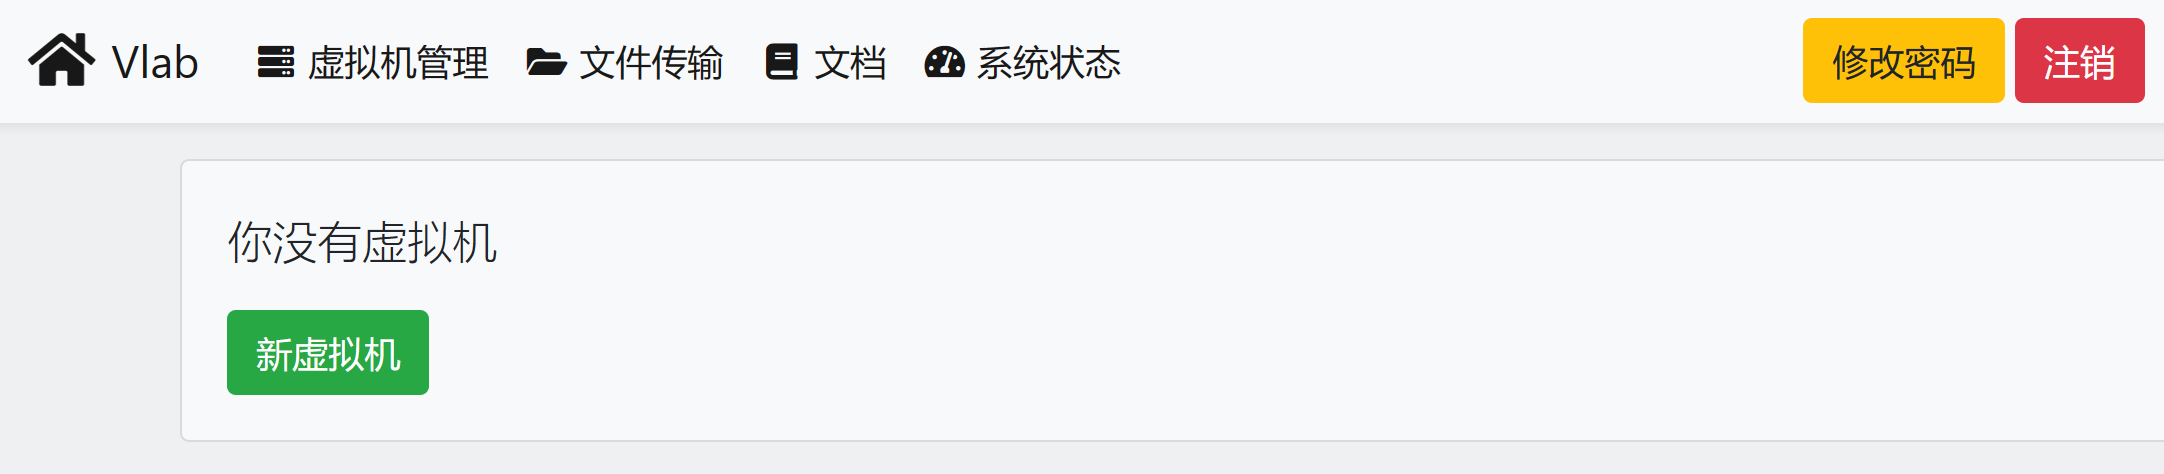
\includegraphics[width=0.85\textwidth]{lab0/1.png}
\end{figure}

\begin{figure}[H]
    \centering
    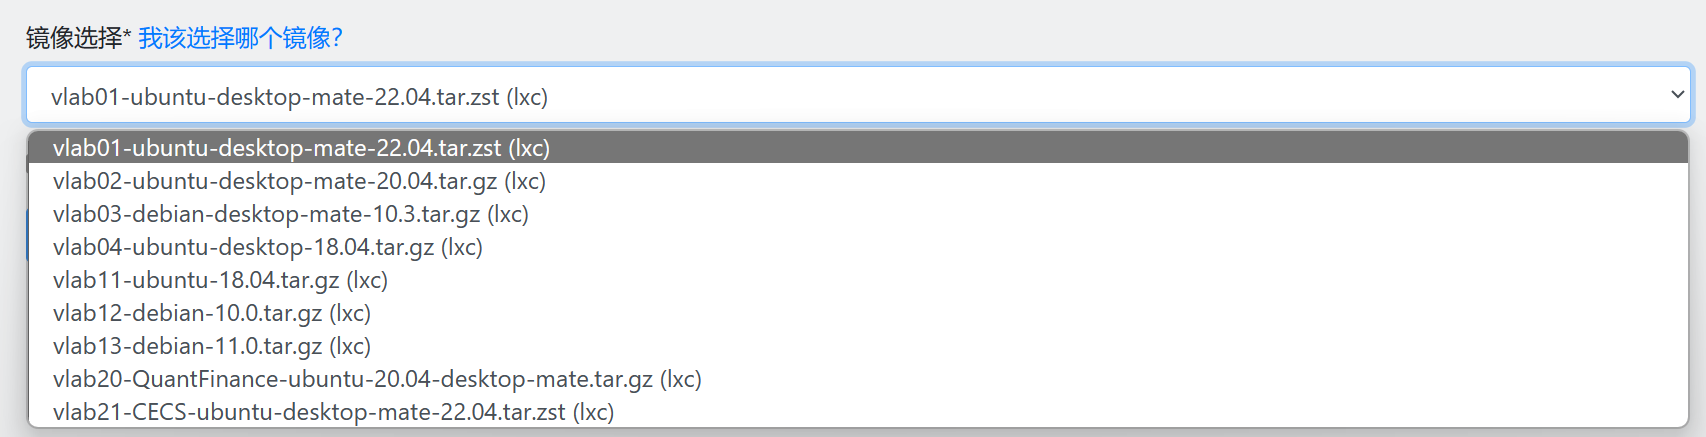
\includegraphics[width=0.85\textwidth]{lab0/2.png}
\end{figure}

云虚拟机上已经配置好了完整的实验环境。使用远程桌面登陆后,即可在左上角的“应用程序 > Vlab 实验软件”中找到需要的实验资源。

\begin{figure}[H]
    \centering
    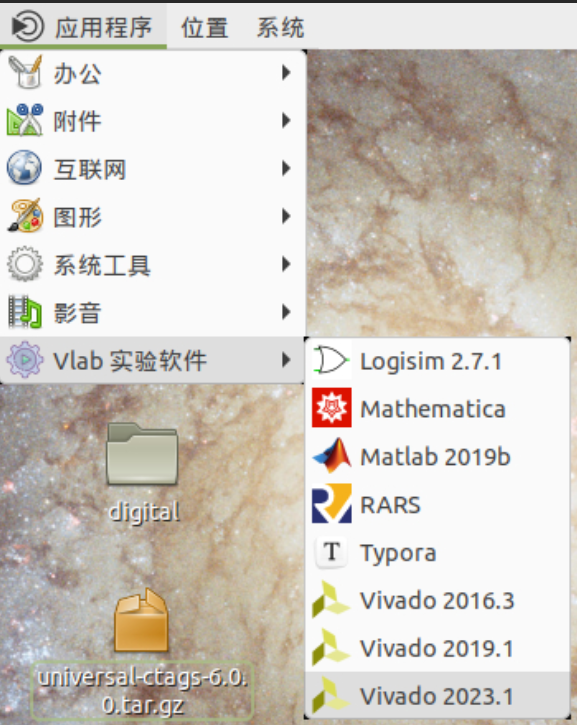
\includegraphics[width=0.3\textwidth]{lab0/3.png}
\end{figure}

\subsection{本地安装}

进入Vivado\href{https://china.xilinx.com/support/download/index.html/content/xilinx/zh/downloadNav/vivado-design-tools/2023-1.html}{下载页面},下载2023.1版本的与您操作系统对应的安装包,接下来以Windows环境下为例进行安装过程介绍。

首先进入下图所示的界面。单击“Next”。

\begin{figure}[H]
    \centering
    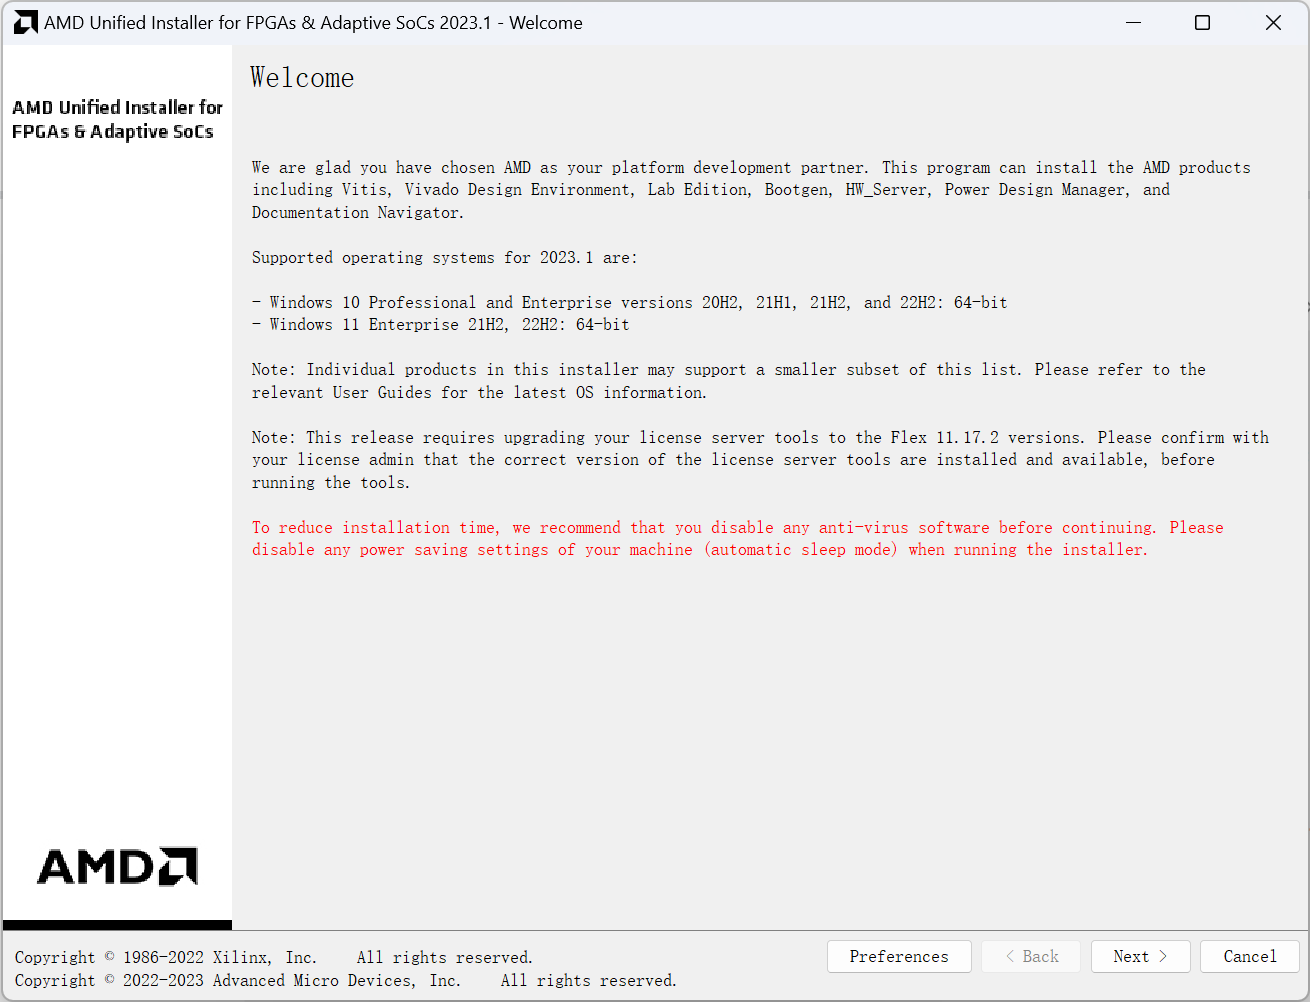
\includegraphics[width=0.85\textwidth]{lab0/4.png}
\end{figure}

接下来是产品界面。单击选择“Vivado”,再单击“Next”以继续安装。

\begin{figure}[H]
    \centering
    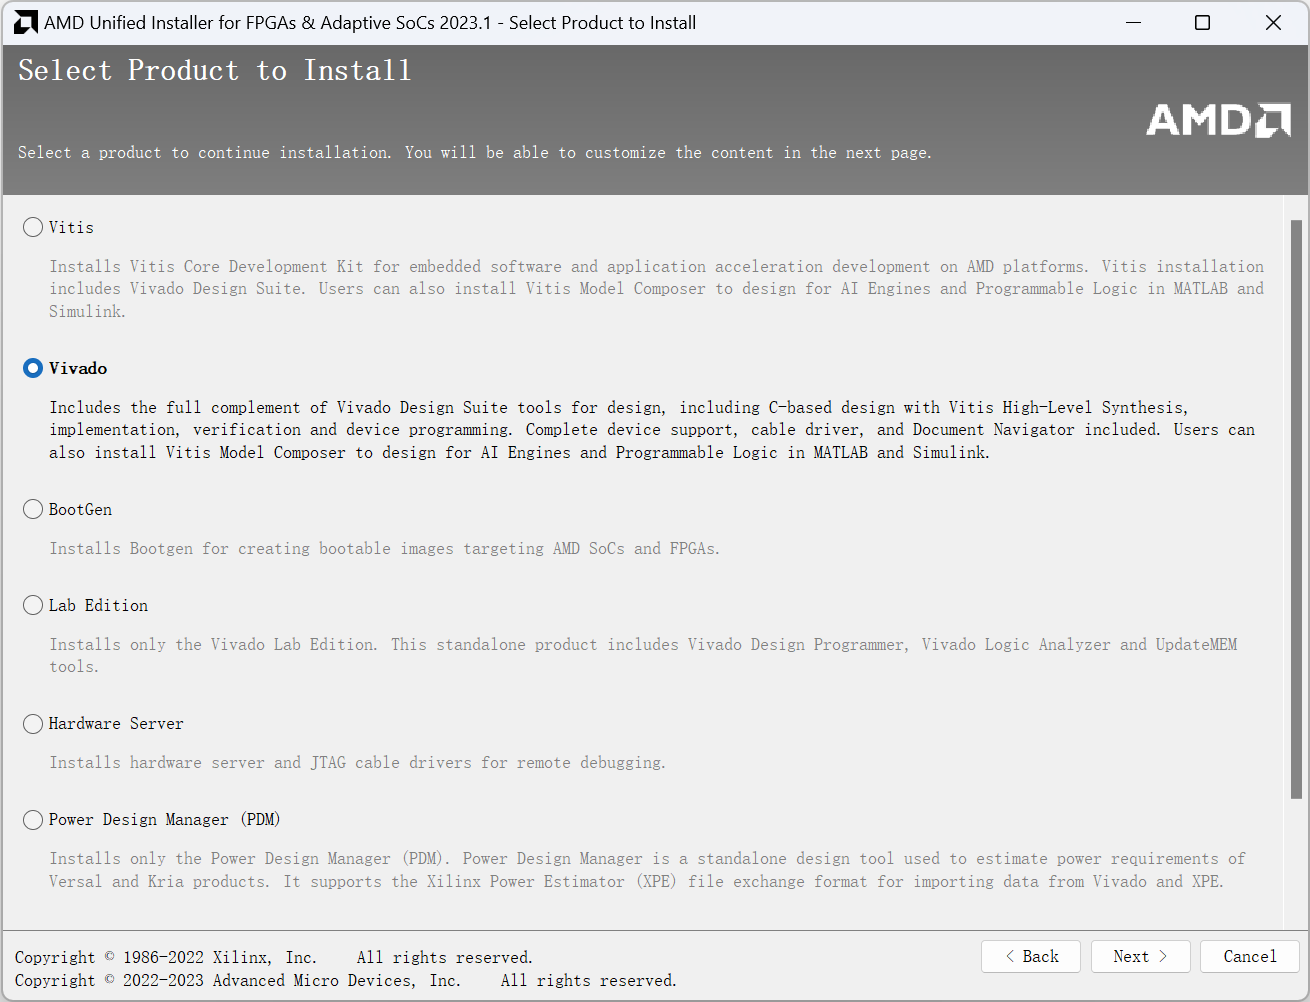
\includegraphics[width=0.85\textwidth]{lab0/5.png}
\end{figure}

选择安装Vivado后,选择标准版本(Standard),单击“Next”以继续安装。

\begin{figure}[H]
    \centering
    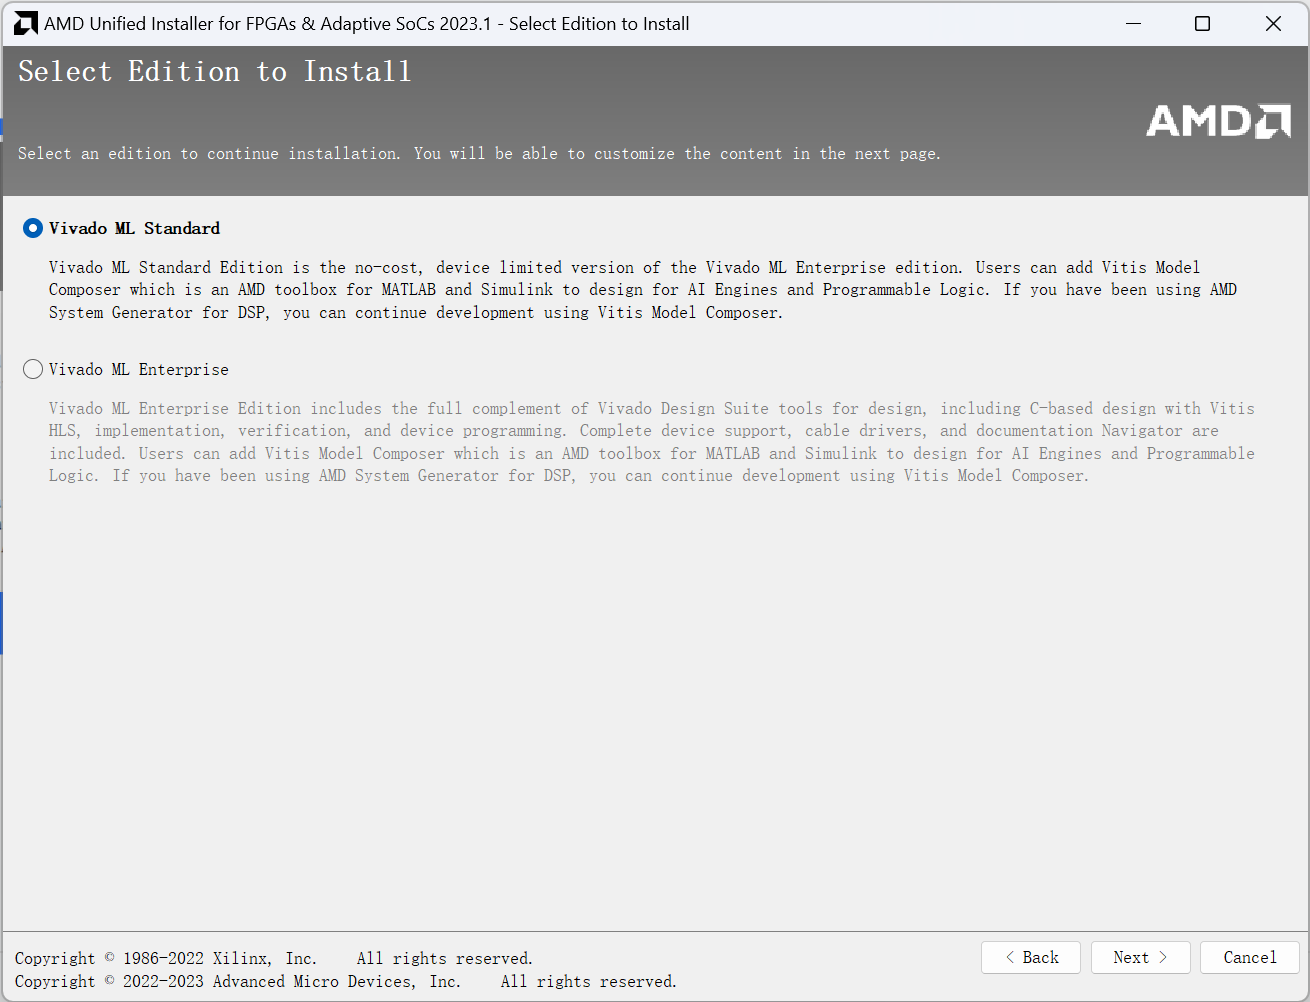
\includegraphics[width=0.85\textwidth]{lab0/6.png}
\end{figure}

接下来的界面是选择安装组件。本课程实验仅需要A7芯片即可,因此为了节省空间,可不装其他功能。设定好相关内容后,单击“Next”以继续安装。

\begin{figure}[H]
    \centering
    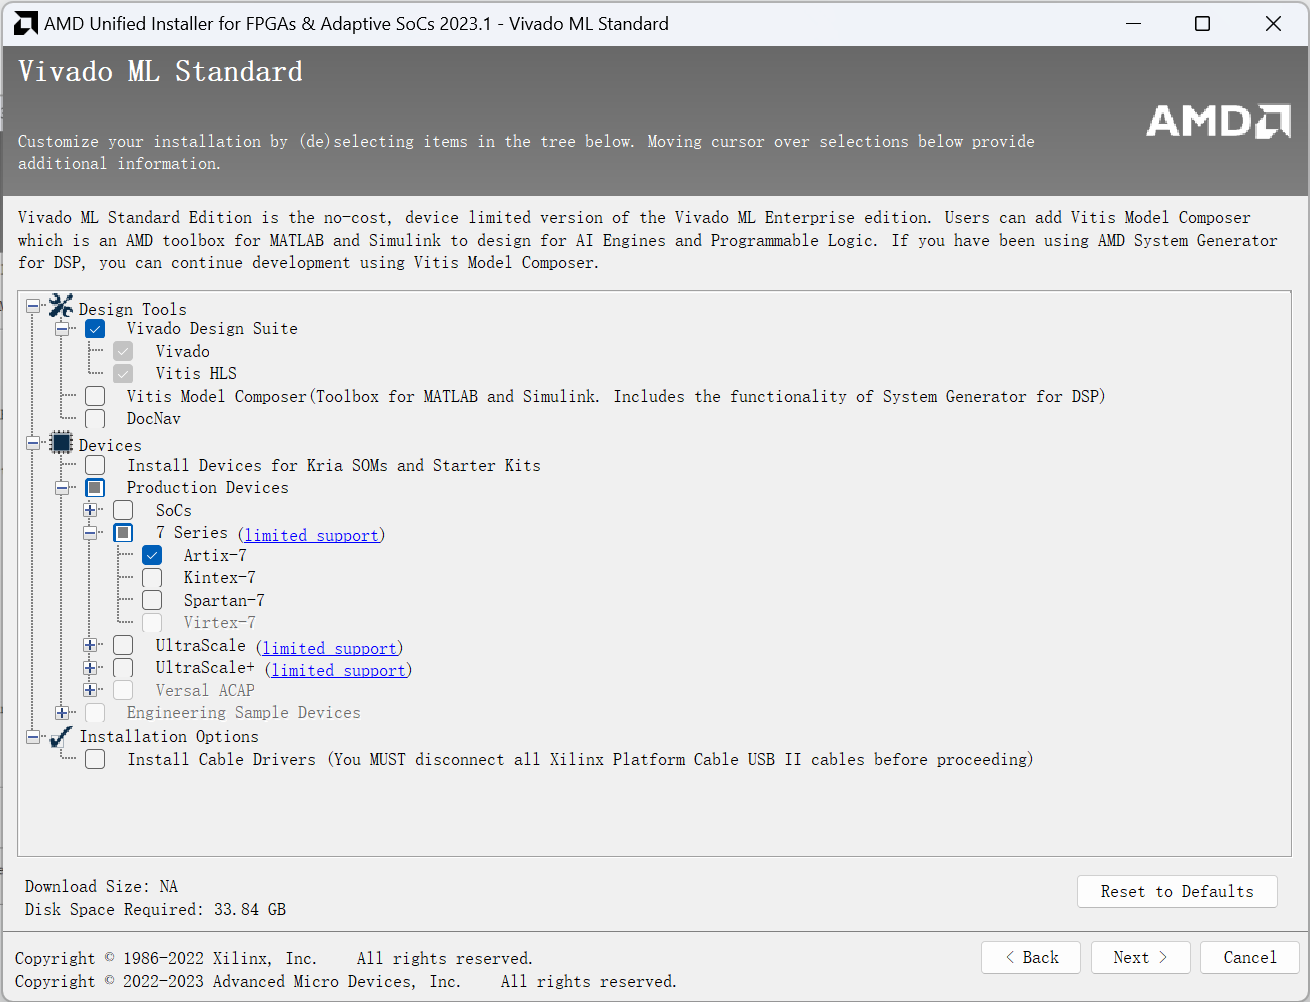
\includegraphics[width=0.85\textwidth]{lab0/7.png}
\end{figure}

接下来需要同意许可协议。设定好相关内容后,单击”Next“以继续安装。

\begin{figure}[H]
    \centering
    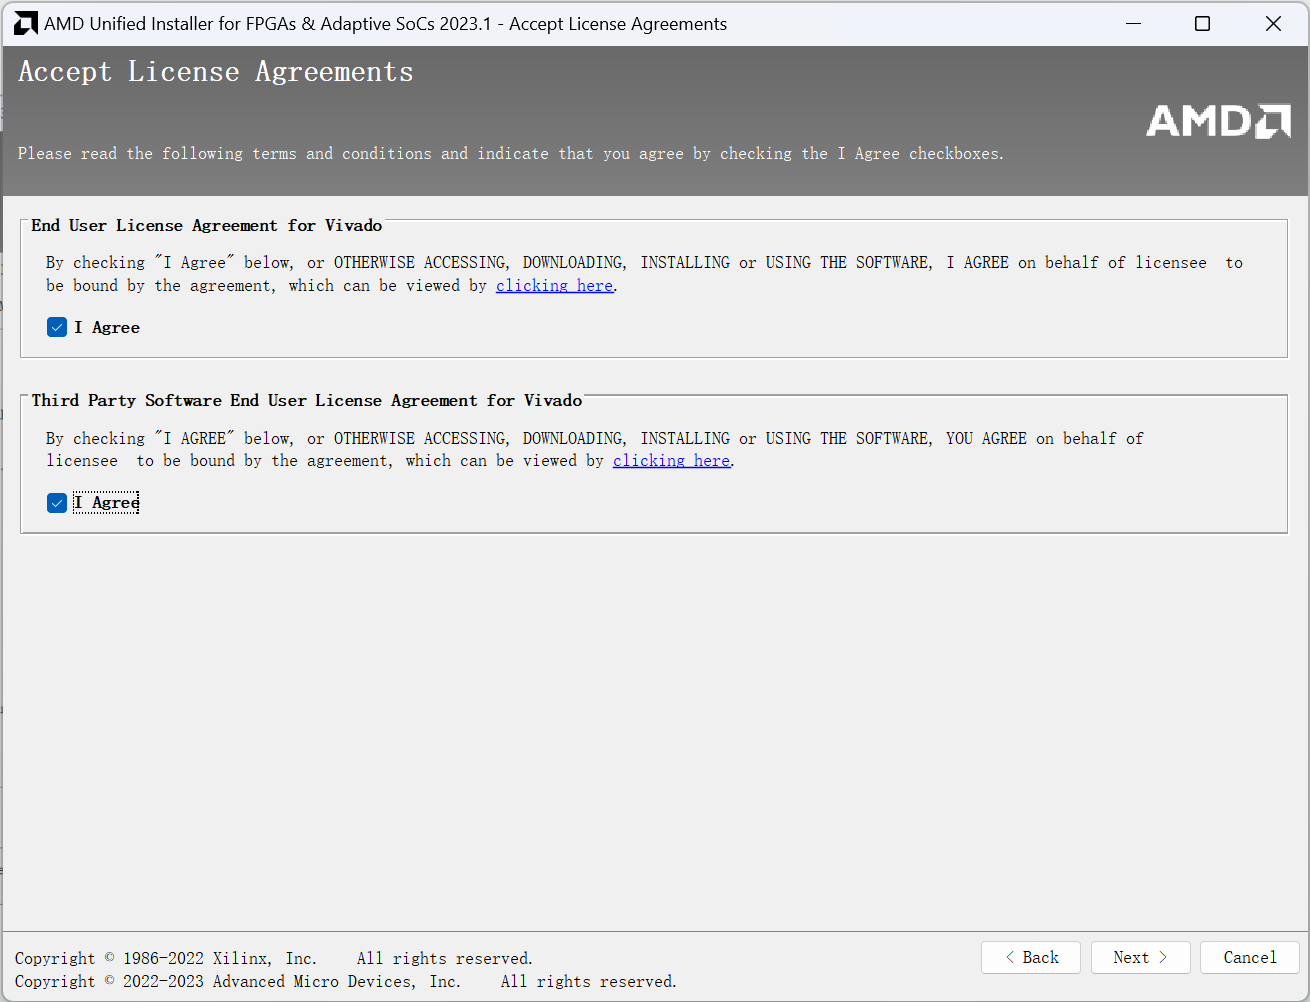
\includegraphics[width=0.85\textwidth]{lab0/8.png}
\end{figure}

接下来是选定安装目录。此时的安装大小超出了 30G,因此不建议直接安装到 C 盘。你可以选择容量充足的位置进行安装。\textbf{注意:安装目录中不能出现中文与空格字符}。设定好相关内容后,单击“Next”以继续安装。

\begin{figure}[H]
    \centering
    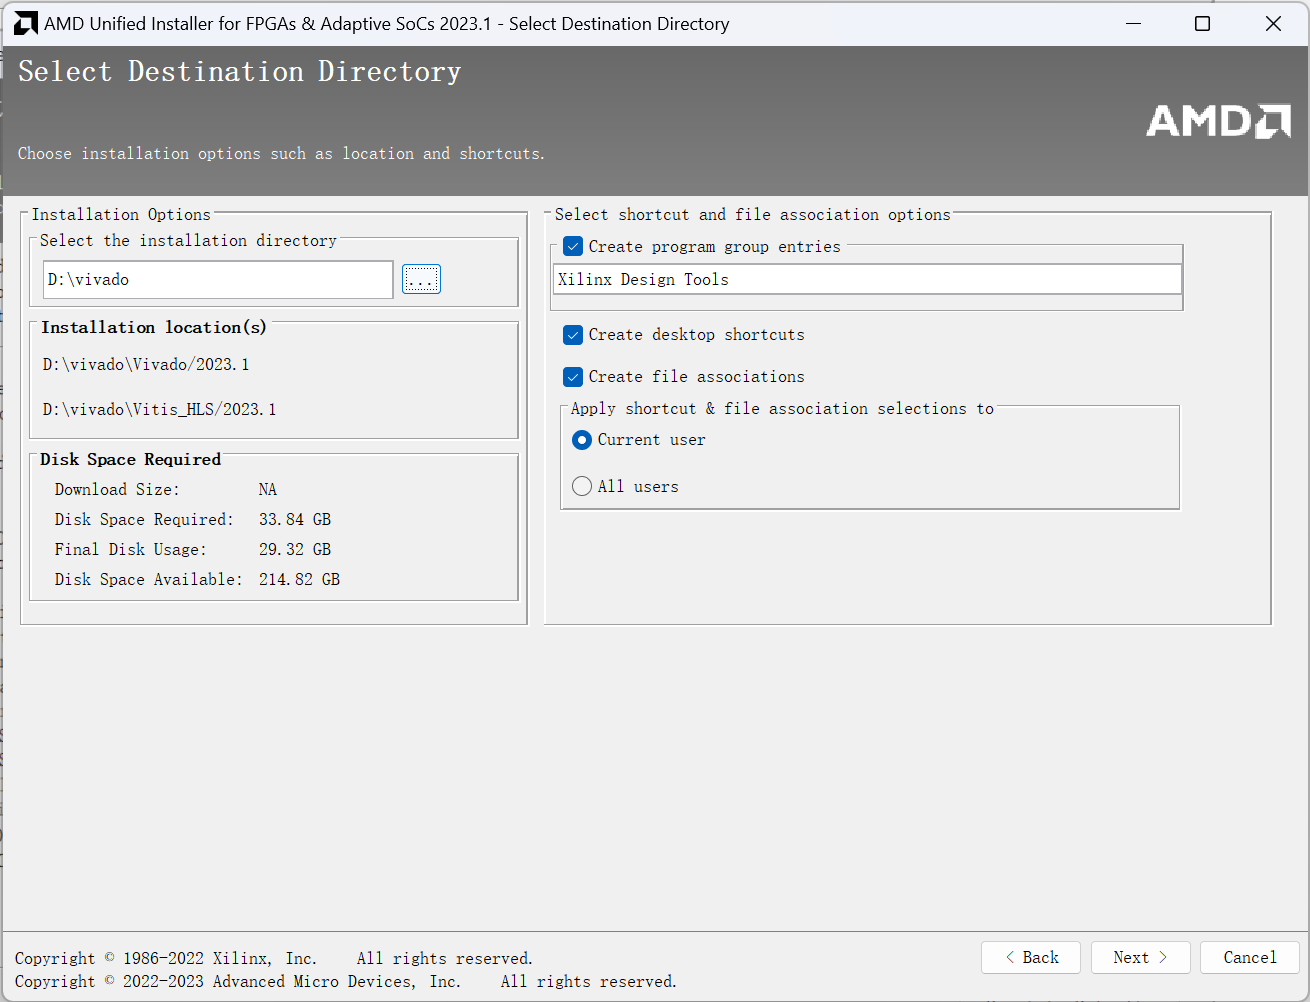
\includegraphics[width=0.9\textwidth]{lab0/9.png}
\end{figure}

最后是安装概览。检查安装信息无误后,单击”Install“以开始安装。

\begin{figure}[H]
    \centering
    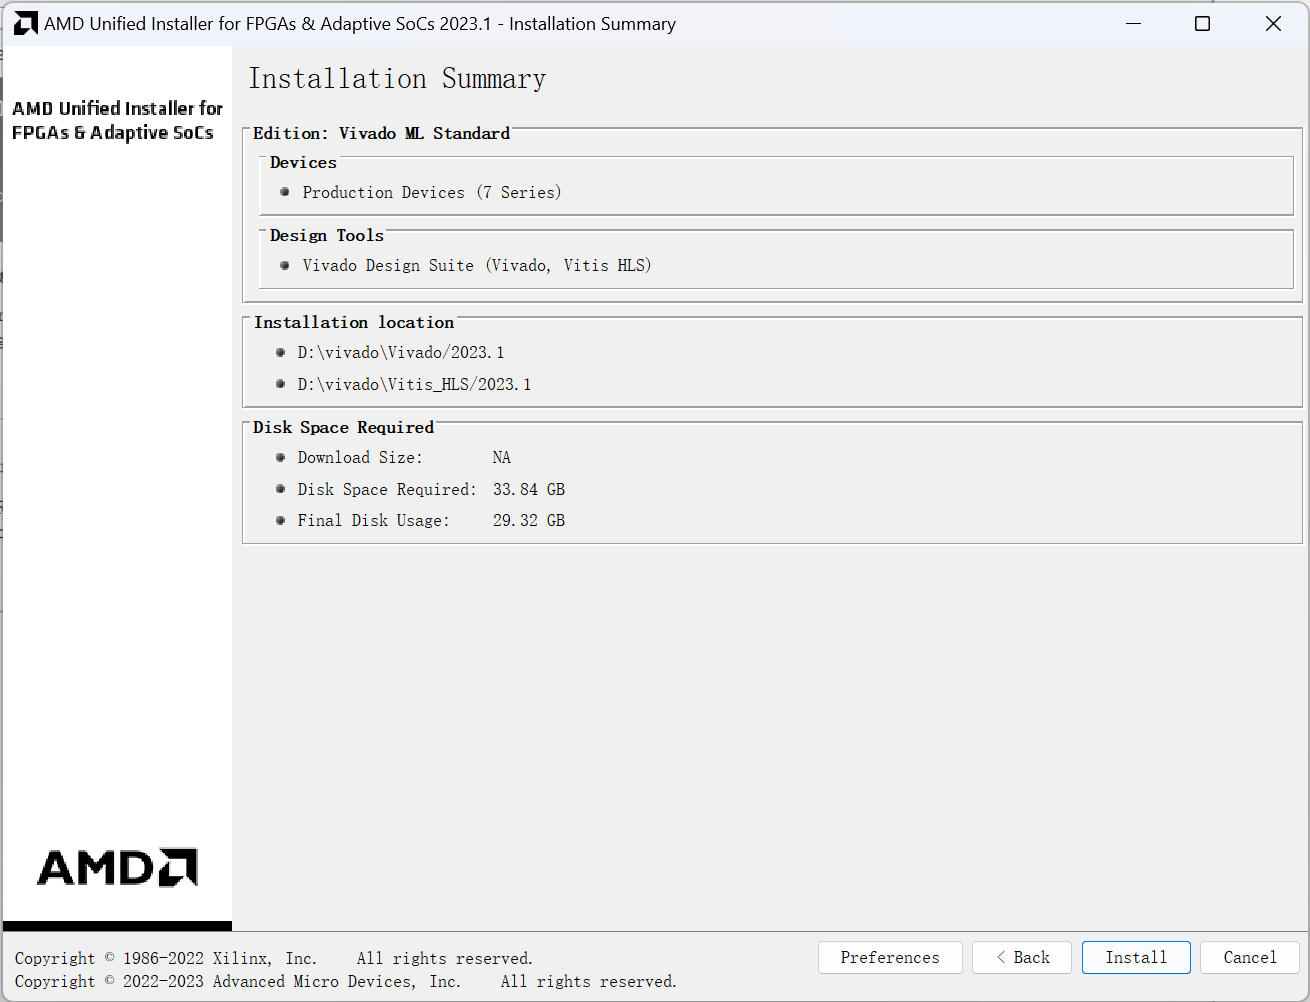
\includegraphics[width=0.85\textwidth]{lab0/10.png}
\end{figure}

\begin{figure}[H]
    \centering
    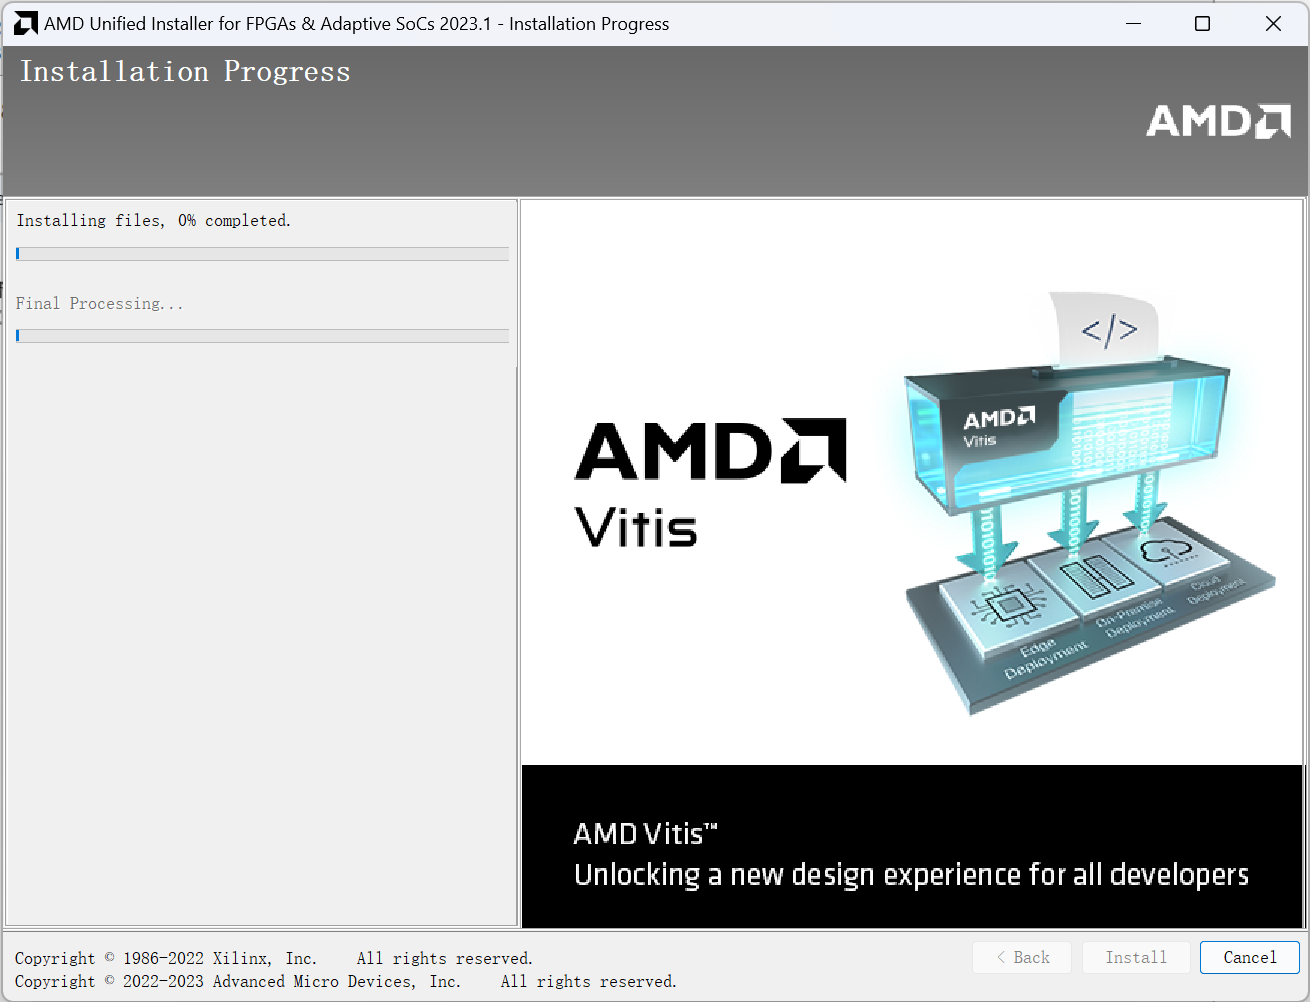
\includegraphics[width=0.85\textwidth]{lab0/11.png}
\end{figure}

当弹出下面的对话框时,表明安装结束。此时点击桌面上的“Vivado 2023.1”图标即可启动 Vivado。

\begin{figure}[H]
    \centering
    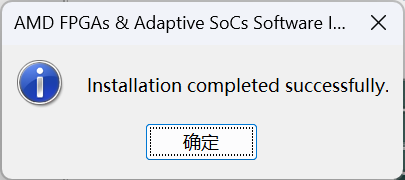
\includegraphics[width=0.5\textwidth]{lab0/12.png}
\end{figure}

\begin{figure}[H]
    \centering
    
\includegraphics[width=0.5\textwidth]{lab0/13.png}
\end{figure}

%------------------------------%

\section{创建项目}

安装完成Vivado之后,启动Vivado,在初始界面上点击“Create Project”。

\begin{figure}[H]
    \centering
    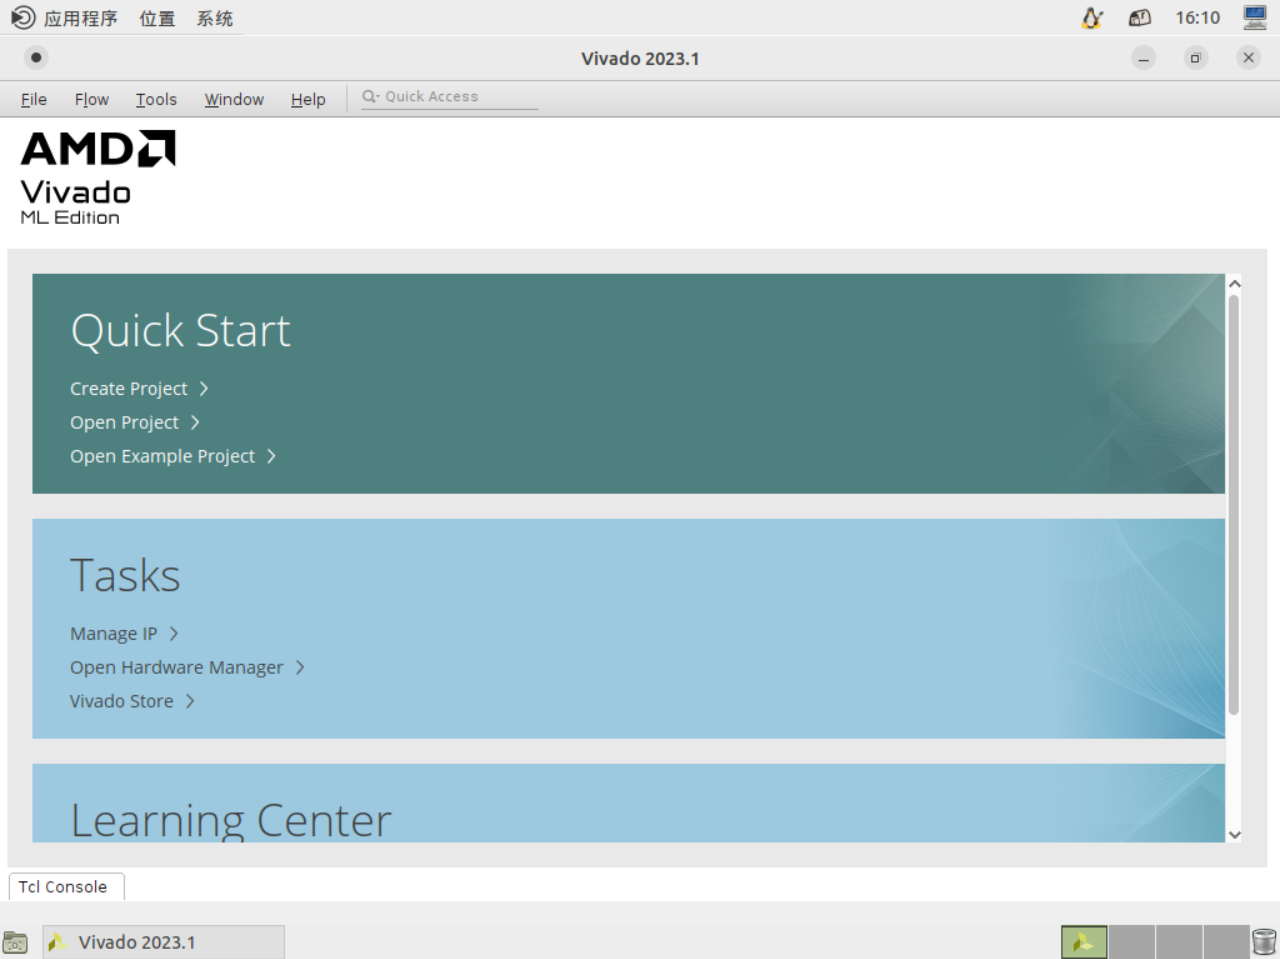
\includegraphics[width=0.85\textwidth]{lab0/14.png}
\end{figure}

一路点击“Next”,直到以下窗口,选择器件型号“xc7a100tcsg324-1”。

\begin{figure}[H]
    \centering
    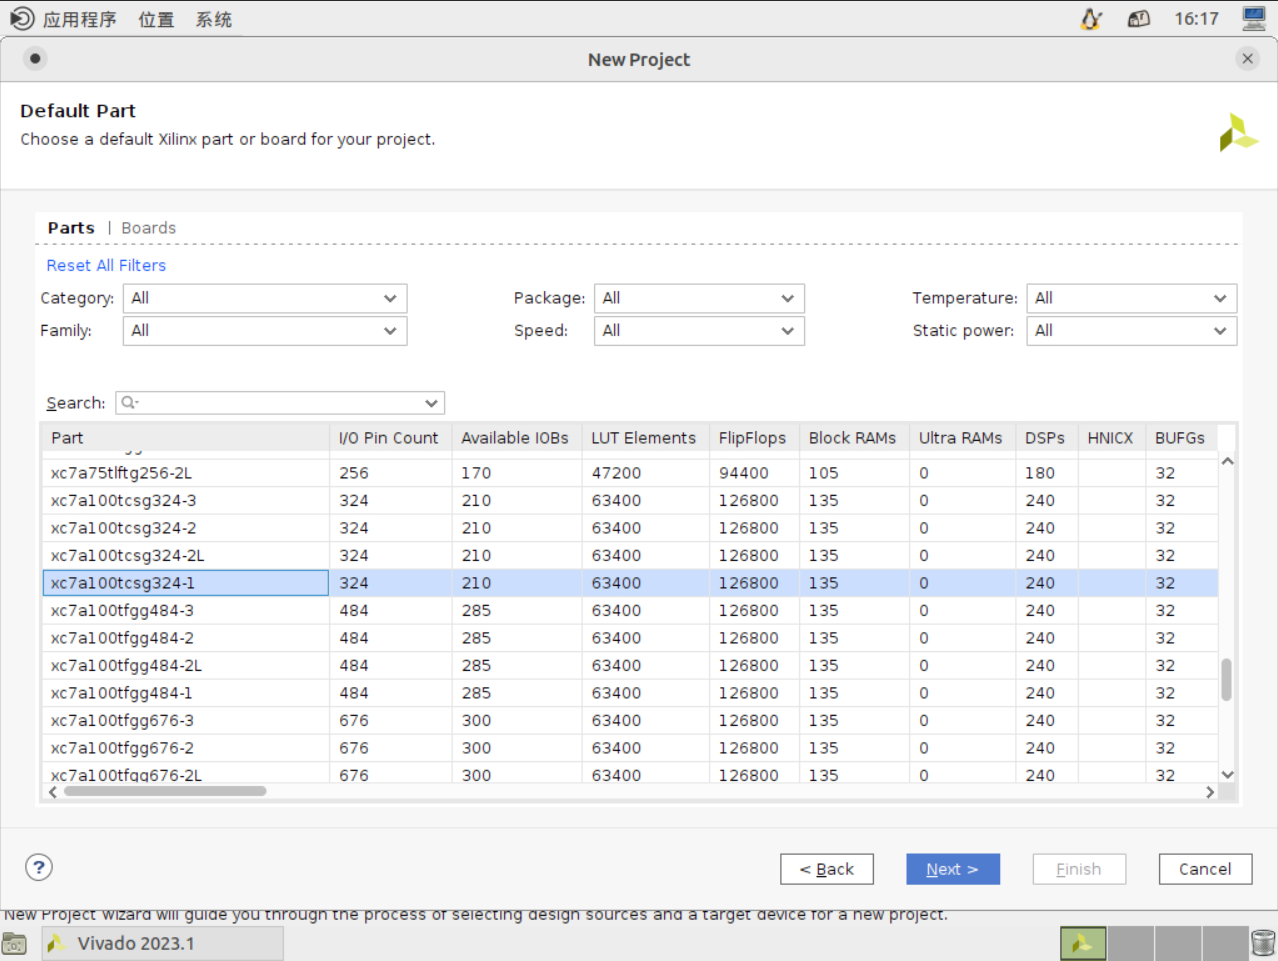
\includegraphics[width=0.85\textwidth]{lab0/15.png}
\end{figure}

然后点击“Next”,完成项目创建。

\begin{figure}[H]
    \centering
    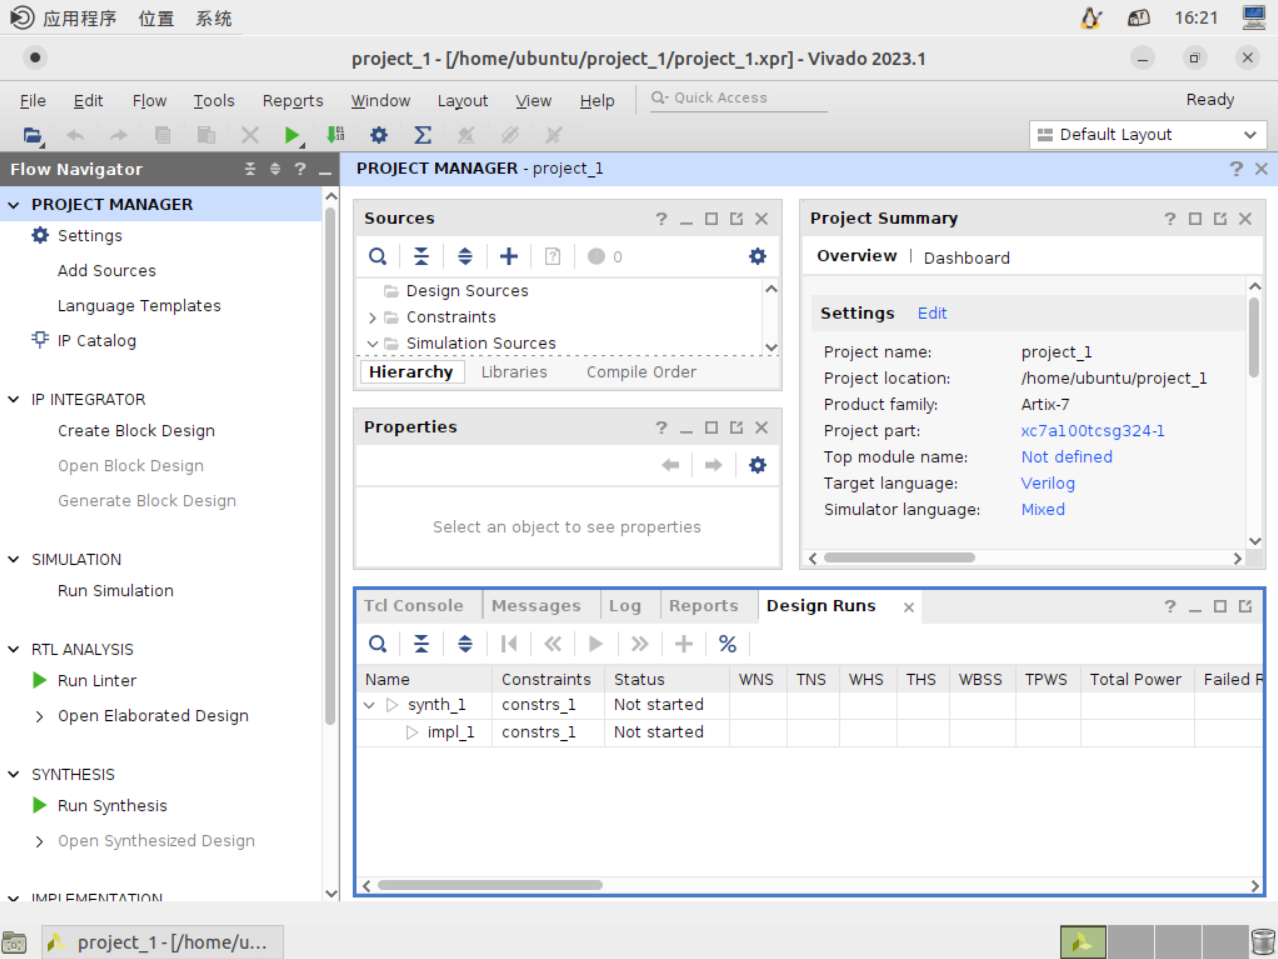
\includegraphics[width=0.85\textwidth]{lab0/16.png}
\end{figure}

从左侧的“Flow Navigator”您可以一目了然地了解Vivado中的FPGA设计流程:

\begin{itemize}
    \item 在“PROJECT MANAGER”视图中,您可以对整个项目的设计进行管理,包括创建/添加源文件、选择语言模板、从IP目录中添加IP等。
    \item 在“IP INTEGRATOR”视图中,您可以创建复杂的子系统设计,以便包含在更高级别的设计或独立设计中。
    \item 在"SIMULATION"视图中,您可以对设计进行行为仿真、功能仿真或时序仿真。
    \item 在“RTL ANALYSIS”视图中,您可以在详细的网表中查看RTL设计,以进行不同设计元素的早期探索和分析。
    \item 在“SYNTHESIS”视图中,您可以查看设计的综合结果并进行分析。
    \item 在“IMPLEMENTATION”视图中,您可以查看综合后的网表在目标设备上的布局和布线结果并进行分析。
    \item 在“PROGRAM AND DEBUG”视图中,您可以生成比特流文件,用于对目标设备的编程,还可以对设备进行调试。
\end{itemize}

%------------------------------%

\section{创建/添加设计文件}

点击“Add Sources”,选择“Add or create design sources”,您可以选择添加或者创建源文件。这里我们创建新的源文件,选择“Create File”,输入文件名“add”,点击“Finish”完成文件创建。创建好的源文件在“Sources”窗口中的“Design Sources”栏目中可以找到。

\begin{figure}[H]
    \centering
    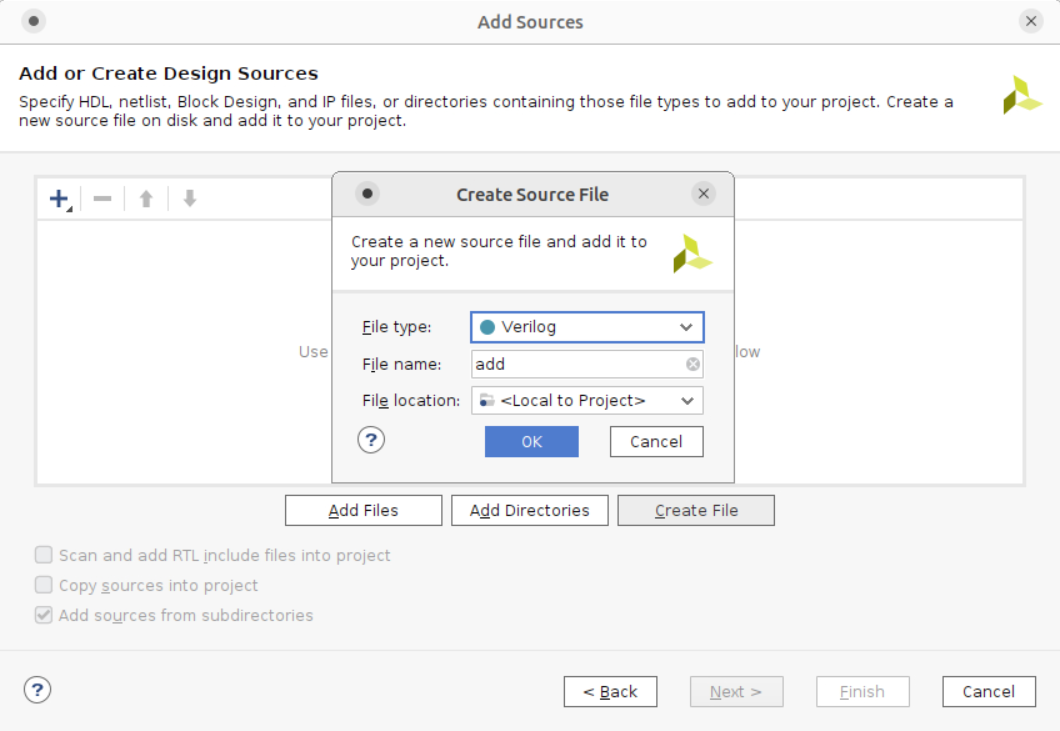
\includegraphics[width=0.8\textwidth]{lab0/17.png}
\end{figure}

\begin{figure}[H]
    \centering
    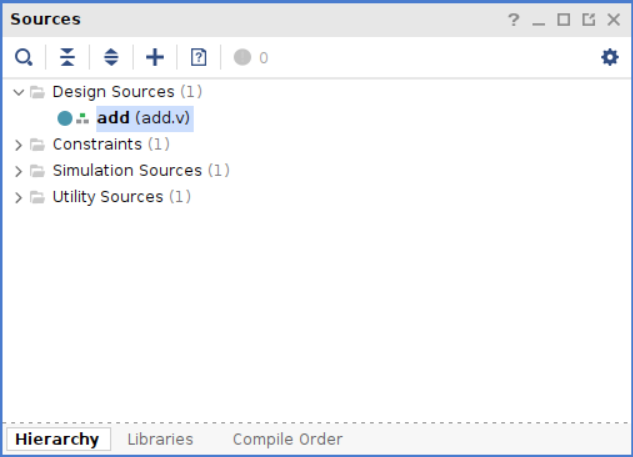
\includegraphics[width=0.6\textwidth]{lab0/18.png}
\end{figure}

双击创建好的“add.v”文件,在右侧的编辑器中输入以下内容作为示例。

\begin{lstlisting}[language=Verilog]
module add (input a,b,c, output s);
    assign s = a + b + c;
endmodule
\end{lstlisting}

综合与实现操作中由约束文件(Constraint File)来指定目标设备的管脚定义等信息,进行设计时按需修改约束文件中的管脚和模块输入输出信号间的绑定。点击左侧“Add Sources”,选择“Add or create constraints”,选择“Create File”,输入文件名“fpgaol”,点击“Finish”完成文件创建。

\begin{figure}[H]
    \centering
    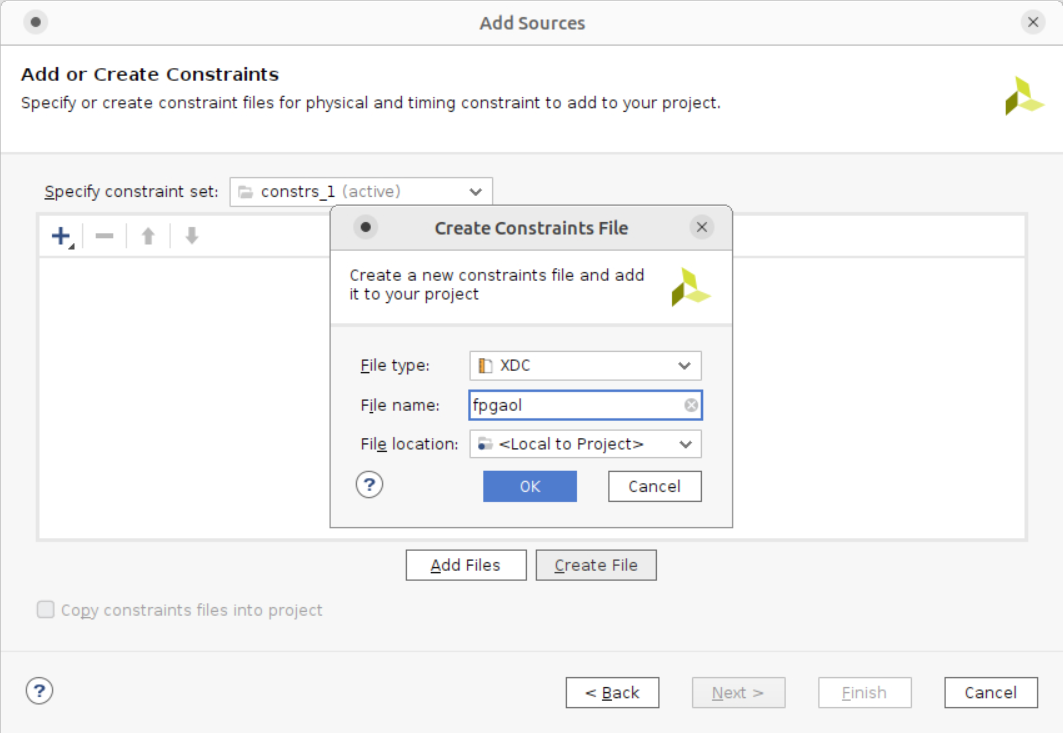
\includegraphics[width=0.8\textwidth]{lab0/19.png}
\end{figure}

\begin{figure}[H]
    \centering
    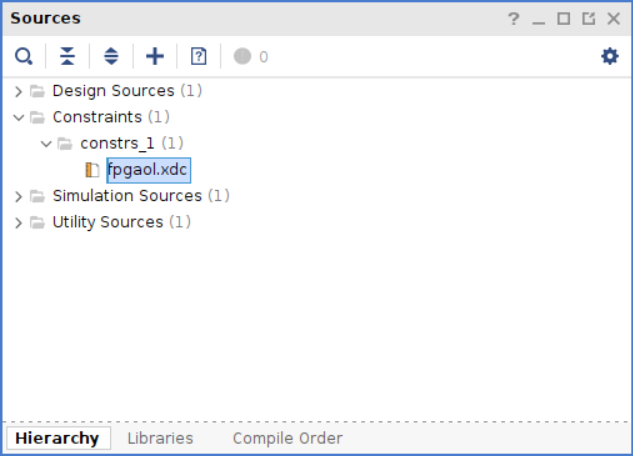
\includegraphics[width=0.6\textwidth]{lab0/20.png}
\end{figure}

在创建的约束文件中添加以下内容。

\begin{lstlisting}[language=Verilog]
set_property -dict { PACKAGE_PIN C17 IOSTANDARD LVCMOS33 } [get_ports { s }];
set_property -dict { PACKAGE_PIN D14 IOSTANDARD LVCMOS33 } [get_ports { a }];
set_property -dict { PACKAGE_PIN F16 IOSTANDARD LVCMOS33 } [get_ports { b }];
set_property -dict { PACKAGE_PIN G16 IOSTANDARD LVCMOS33 } [get_ports { c }];
\end{lstlisting}

%------------------------------%

\section{仿真}

为了避免上板时代码错误导致的烧板,或是减少调试的时间,您应该在上板之前执行仿真。

首先创建仿真文件,点击“Add Sources”,选择“Add or create simulation sources”。创建新的仿真文件,选择“Create File”,输入文件名“add\_tb”(习惯上一个源文件对应的仿真文件的命名即添加后缀“\_tb”),点击“Finish”完成文件创建。创建好的源文件在“Sources”窗口中的“Simulation Sources/sim\_1”栏目中可以找到。

\begin{figure}[H]
    \centering
    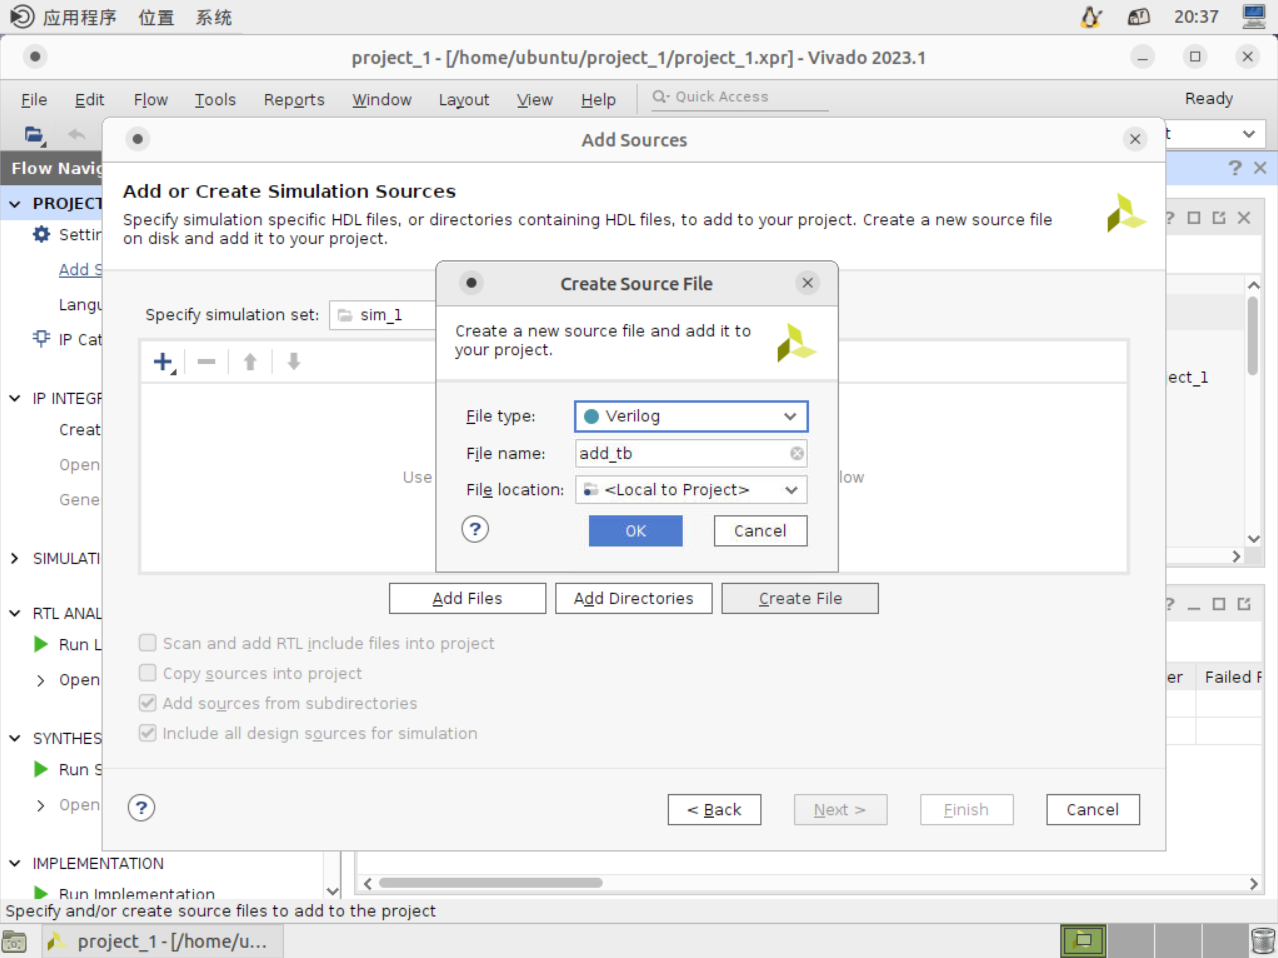
\includegraphics[width=0.8\textwidth]{lab0/21.png}
\end{figure}

\begin{figure}[H]
    \centering
    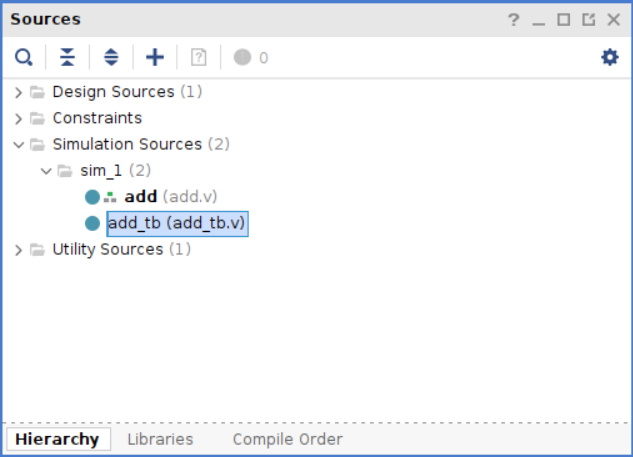
\includegraphics[width=0.6\textwidth]{lab0/22.png}
\end{figure}

双击创建好的“add\_tb.v”文件,在右侧的编辑器中输入以下内容作为示例。

\begin{lstlisting}[language=Verilog]
module add_tb;
    reg a,b,c;
    wire d;
    add u_add(a,b,c,d);
    initial begin
        a=0; b=0; c=0;
        #5; a=1;
        #5; b=1;
        #5; c=1;
    end
endmodule
\end{lstlisting}

点击左侧的“SIMULATION > Run Simulation > Run Behavioral Simulation”执行行为仿真,结束后可以在右侧的窗口查看仿真的波形图。

\begin{figure}[H]
    \centering
    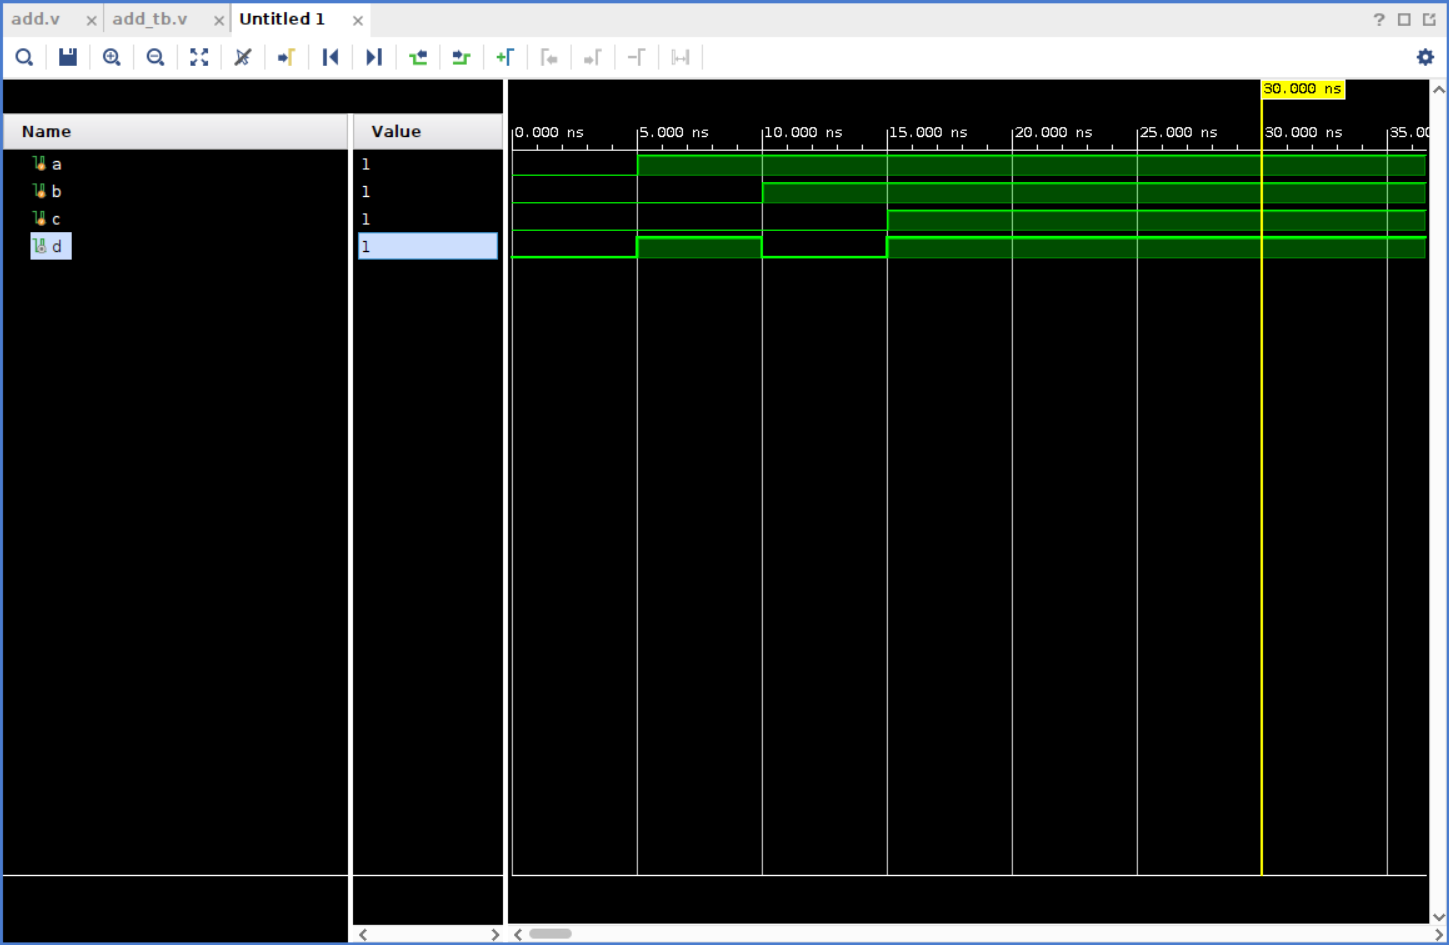
\includegraphics[width=0.8\textwidth]{lab0/23.png}
\end{figure}

通过对比不同阶段的输入和对应的输出波形,就能初步判断代码的功能是否实现正确。上述运行的行为仿真(Behavioral Simulation)只能确保逻辑上近乎正确,而功能仿真(Functional Simulation)和时序仿真(Timing Simulation)则是在考虑了元件差异和信号延迟等因素后进行的仿真。本课程实验中主要以行为仿真作为主要的纠错手段。

%------------------------------%

\section{RTL分析}

点击左侧的“RTL ANALYSIS > Run Linter”,即可进行一个较高级别的代码检查。检查完毕后,下方的Linter栏目中会给出一些可能的警告。值得注意的是,Linter给出的警告不一定会影响设计正确性,而出于设计的规范性和鲁棒性的考虑,应尽量正确处理这里给出的警告。

\begin{figure}[H]
    \centering
    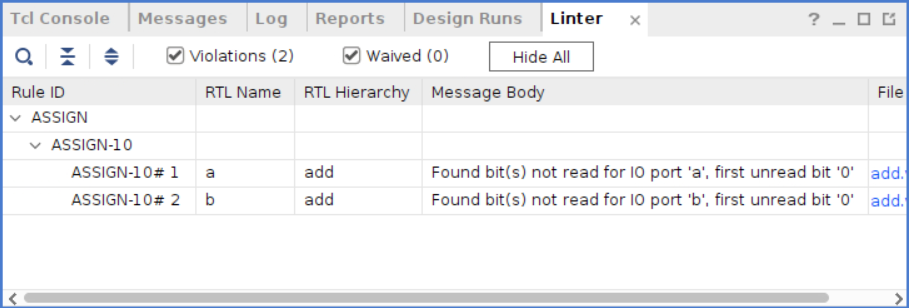
\includegraphics[width=0.85\textwidth]{lab0/24.png}
\end{figure}

点击左侧的“RTL ANALYSIS > Open Elaborated Design”,可以在右侧窗口看到源代码对应电路的逻辑框图,这便于您更快找出源代码中的设计错误。

\begin{figure}[H]
    \centering
    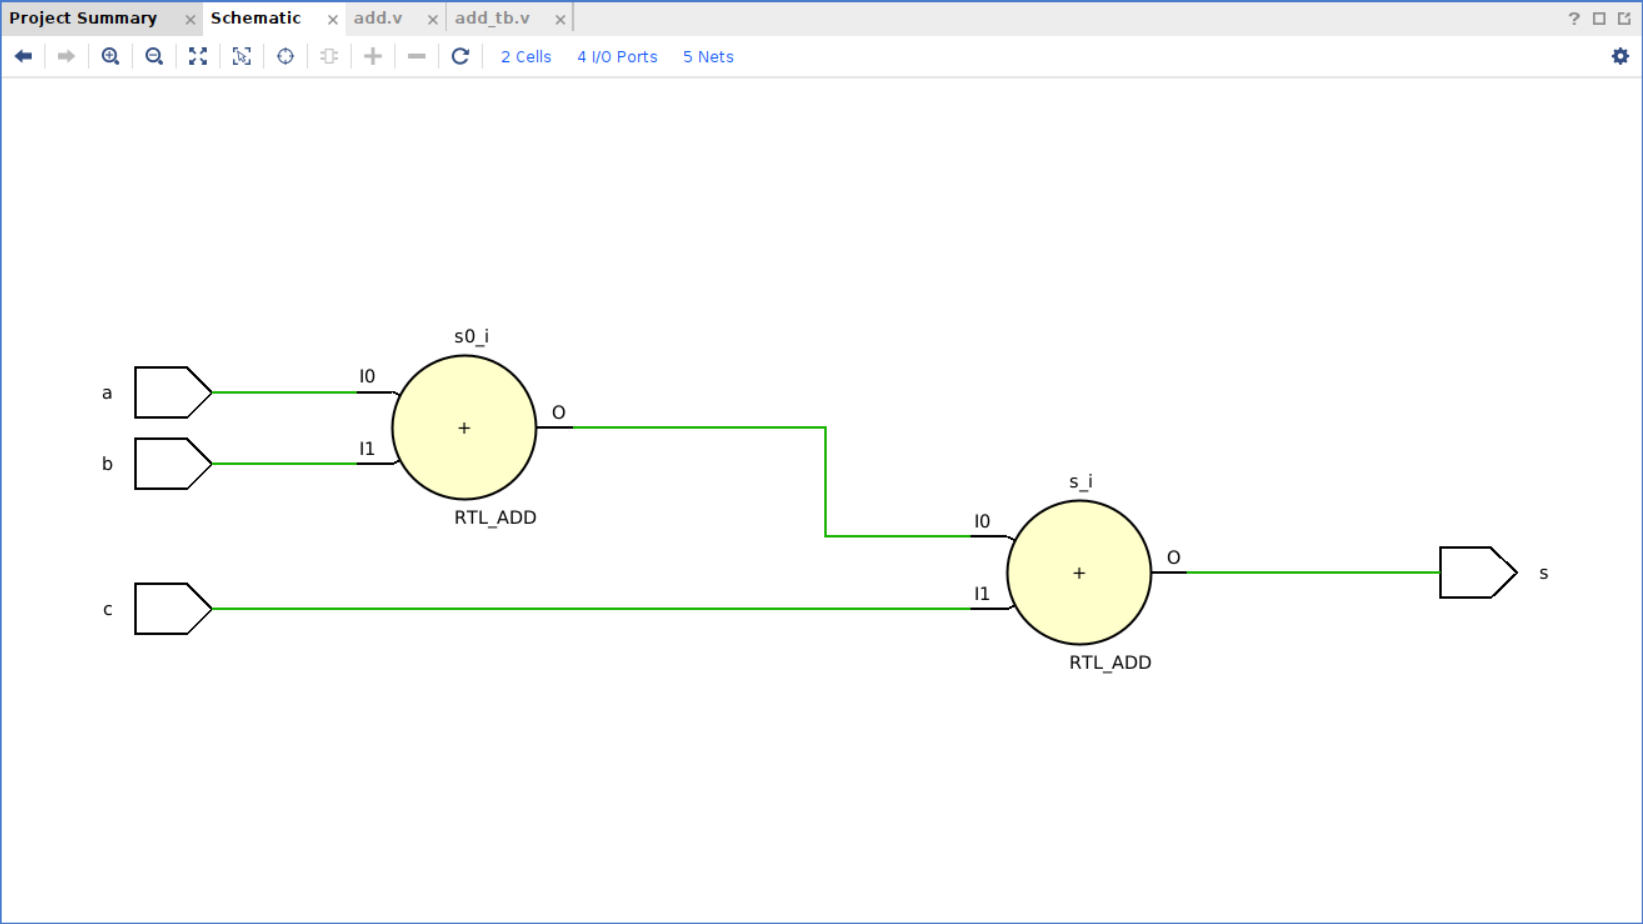
\includegraphics[width=0.85\textwidth]{lab0/25.png}
\end{figure}

%------------------------------%

\section{综合}

执行综合(Synthesis)就是将HDL代码编译为具有门级电路关系的逻辑网表,再通过技术映射转换为使用FPGA基本元件表示的逻辑网表。这一过程中,综合器会执行多项代码优化和电路优化,也可能会给出新的警告或错误,如逻辑环路和多驱动等。

\begin{figure}[H]
    \centering
    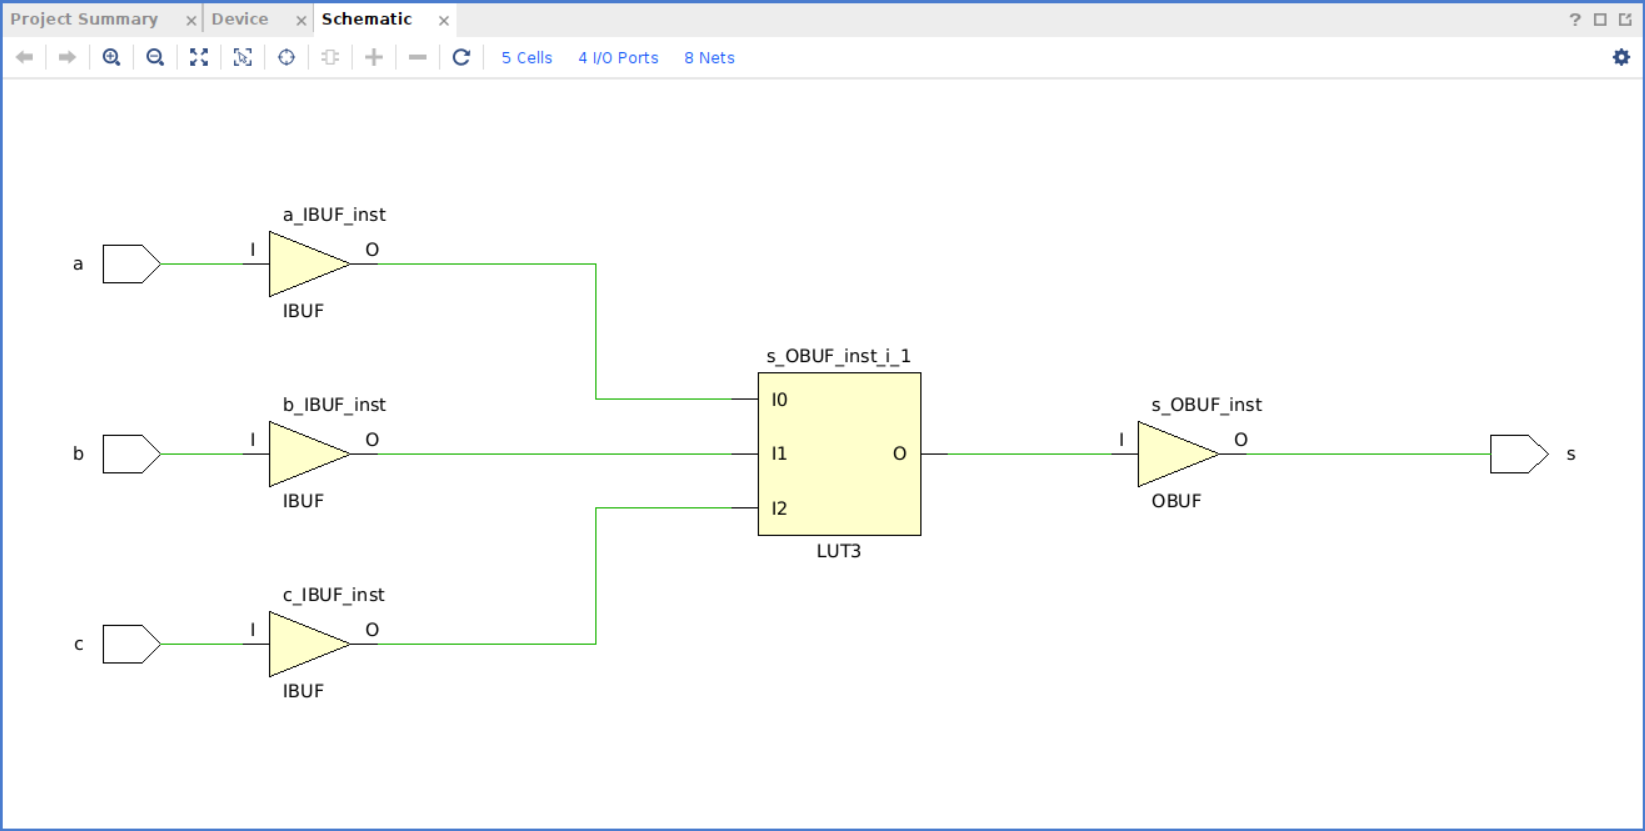
\includegraphics[width=0.85\textwidth]{lab0/26.png}
\end{figure}

点击左侧的“SYNTHESIS > Run Synthesis”执行综合操作。综合结束后点击“SYNTHESIS > Open Synthesized Design > Schematic”,可以在右侧的窗口查看使用FPGA基本元件表示的电路图。

\begin{figure}[H]
    \centering
    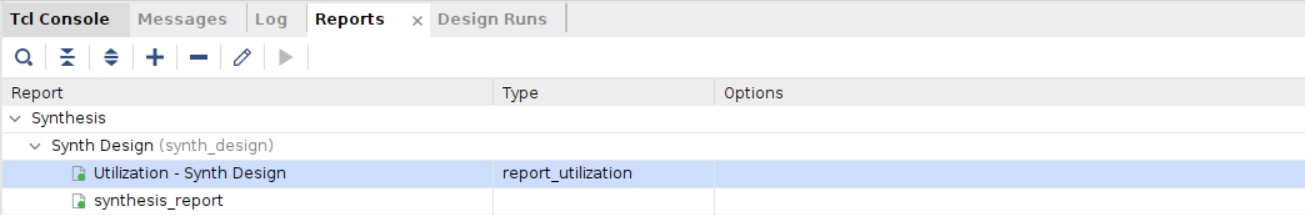
\includegraphics[width=0.85\textwidth]{lab0/27.png}
\end{figure}

%------------------------------%

\section{实现}

实现(Implementation)主要包括两个步骤:布局(Placement)和布线(Routing)。实现操作根据综合操作生成的逻辑网表在特定的设备上进行布局布线,生成特定的物理网表。

点击左侧的“IMPLEMENTATION > Run Implementation“执行实现操作。实现结束后点击”IMPLEMENTATION > Open Implementation Design > Schematic“, 可以在右侧窗口查看实际使用的FPGA基本元件表示的电路图。

\begin{figure}[H]
    \centering
    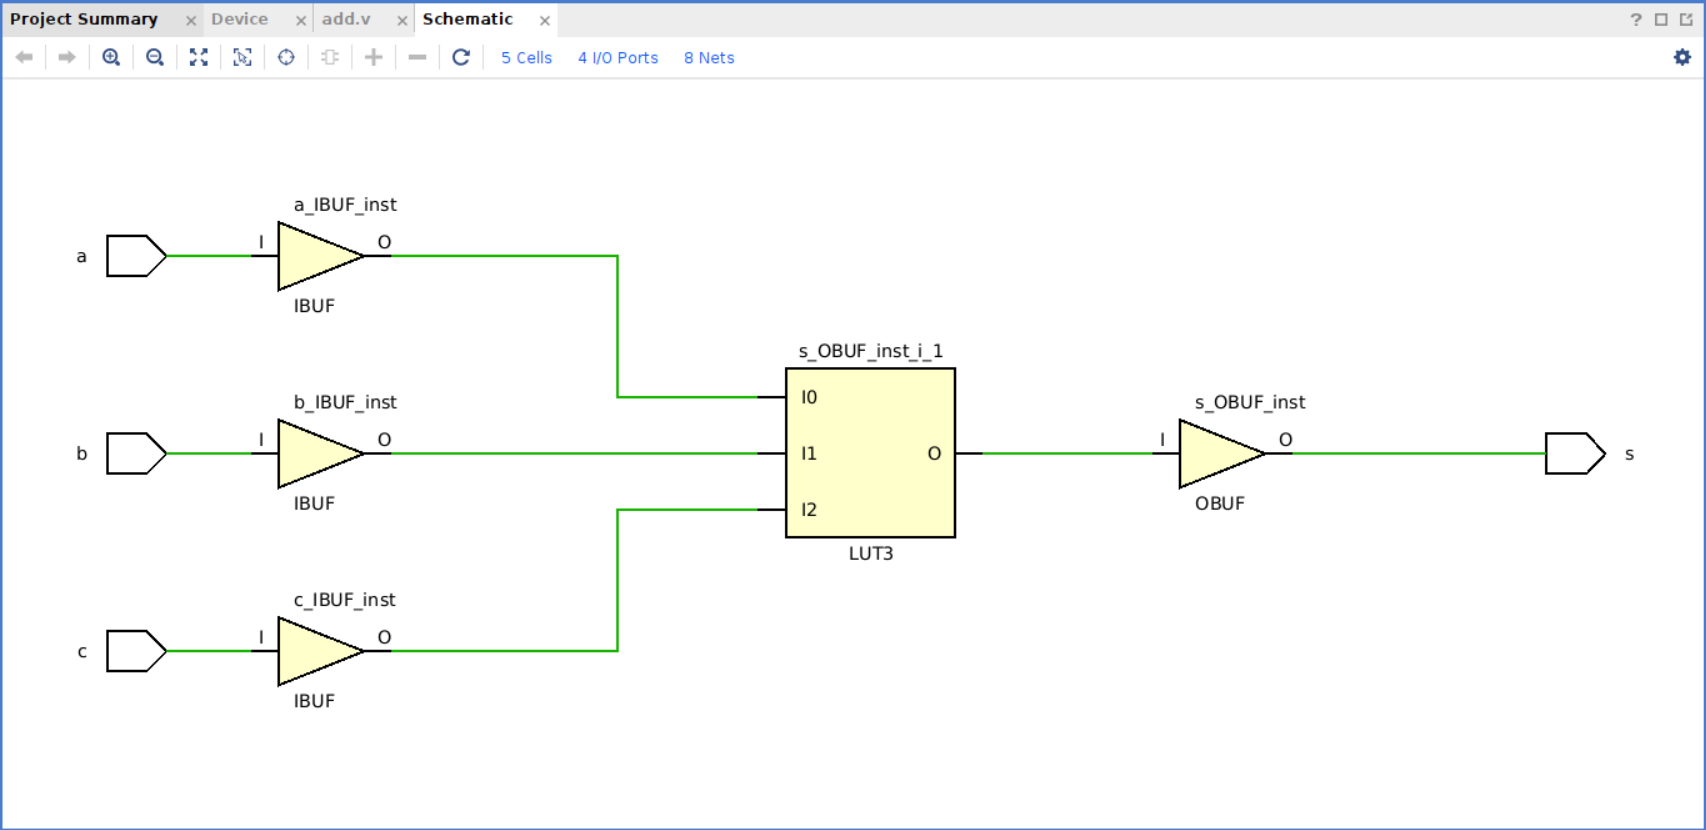
\includegraphics[width=0.85\textwidth]{lab0/28.png}
\end{figure}

您还可在”Device“标签查看目标设备上布局布线后的结果。(为了更好说明,这里展示其他设计。)

\begin{figure}[H]
    \centering
    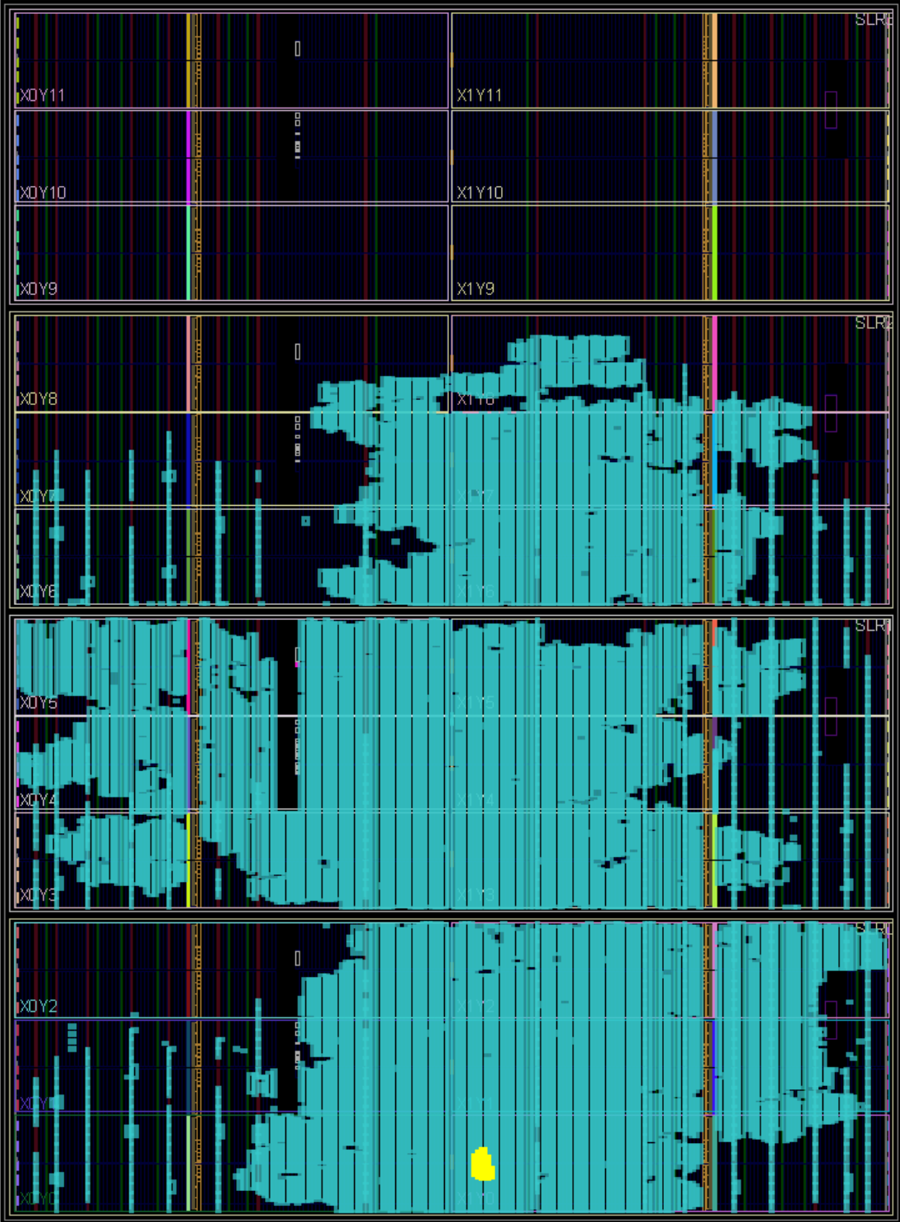
\includegraphics[width=0.5\textwidth]{lab0/29.png}
\end{figure}

执行实现操作后,我们可以得到更为准确的评估信息,如各部件的资源使用率、设计约束检查、功耗和时序等。同时,可能会有更多的问题出现,如时序不满足(逻辑电路过长)等。详细的信息均可在左侧的”IMPLEMENTATION“栏目中获取。

\begin{figure}[H]
    \centering
    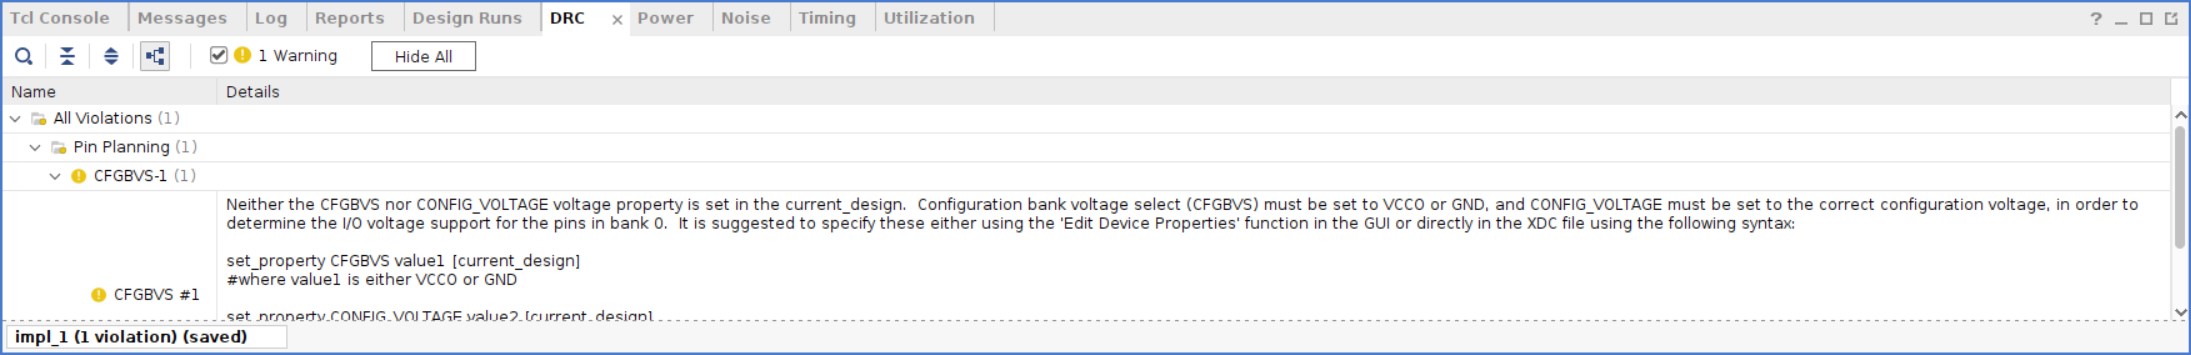
\includegraphics[width=\textwidth]{lab0/30.png}
\end{figure}

\begin{figure}[H]
    \centering
    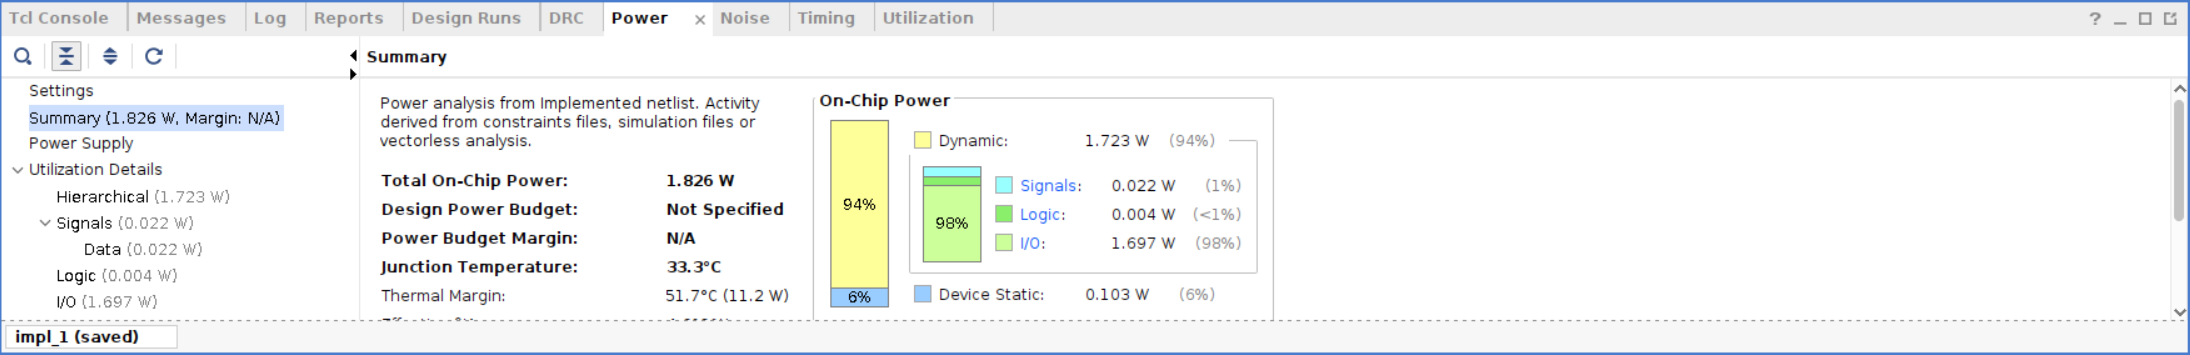
\includegraphics[width=\textwidth]{lab0/31.png}
\end{figure}

\begin{figure}[H]
    \centering
    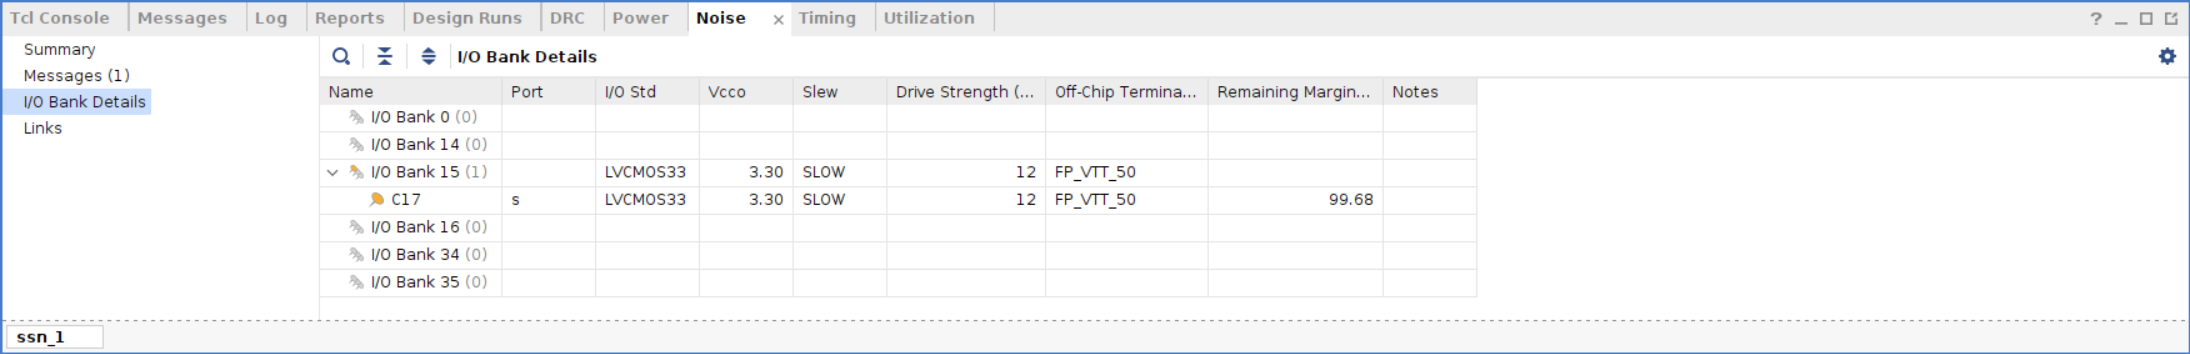
\includegraphics[width=\textwidth]{lab0/32.png}
\end{figure}

\begin{figure}[H]
    \centering
    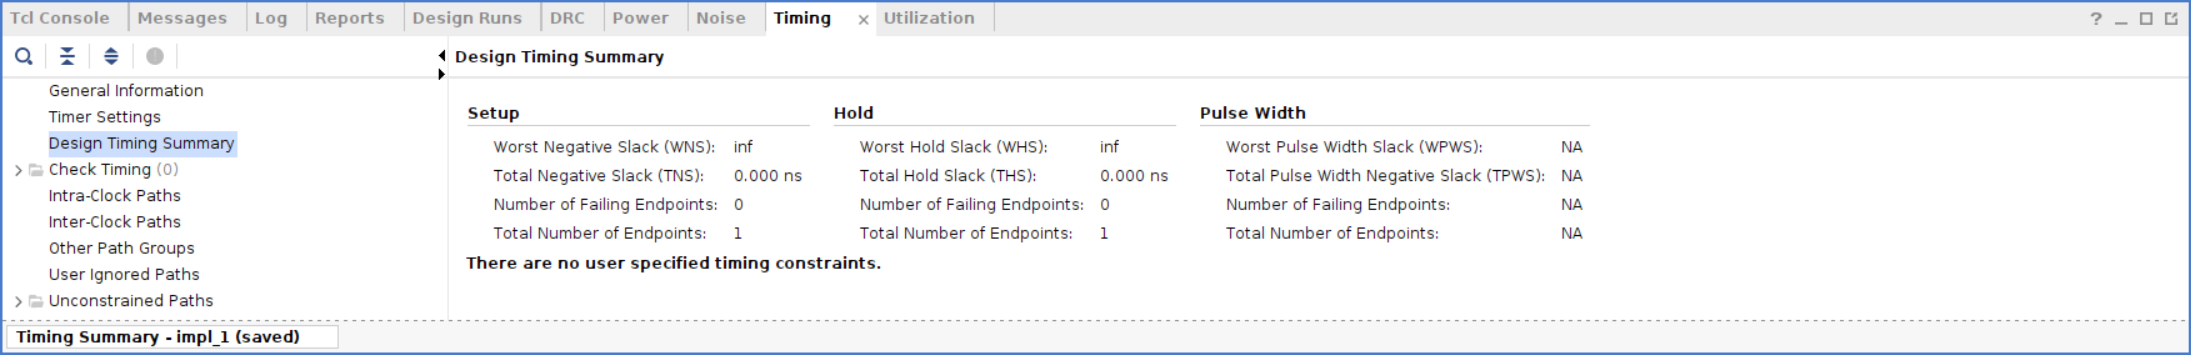
\includegraphics[width=\textwidth]{lab0/33.png}
\end{figure}

\begin{figure}[H]
    \centering
    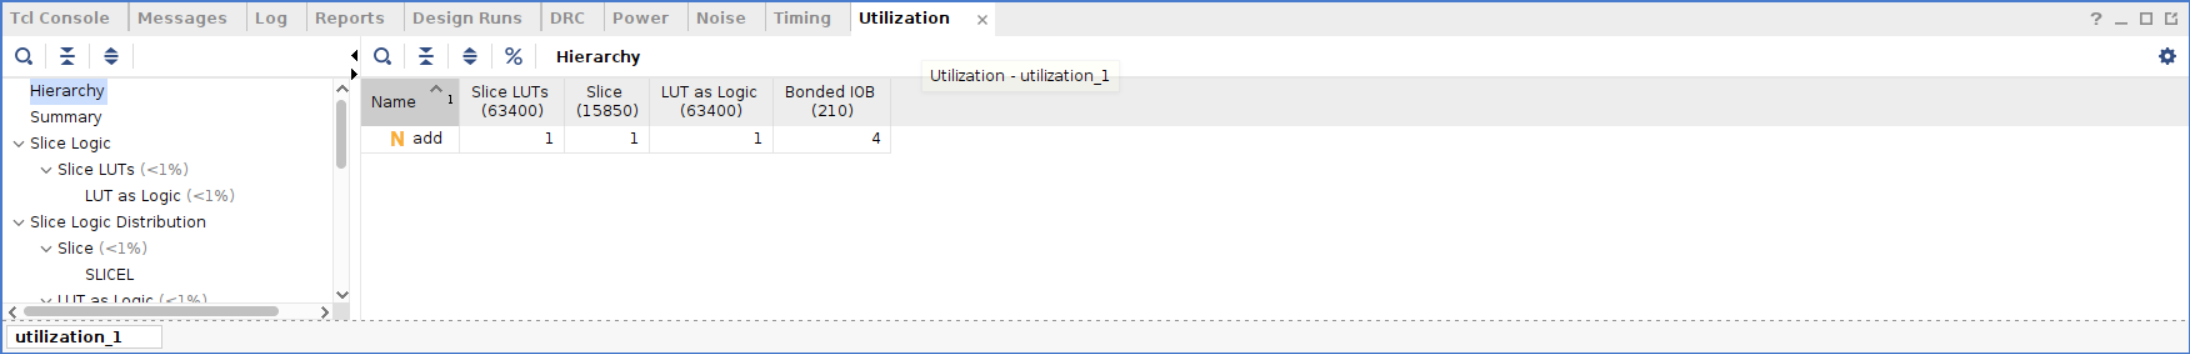
\includegraphics[width=\textwidth]{lab0/34.png}
\end{figure}

%------------------------------%

\section{生成比特流}

点击左侧的”PROGRAM AND DEBUG > Generate Bitstream“即可生成比特流,生成的比特流文件位于“<prj\_loc>/project\_1/project\_1.runs/impl\_1/add.bit”。准备好比特流文件后便可以烧录到板卡上,或上传到云端设备中。

%------------------------------%

\section{上板测试}

本课程实验使用Vlab提供的FPGAOL实验环境,登录后点击“acquire”申请一块云端FPGA板卡,每次使用FPGA资源的时间默认为10分钟,超时后即被释放,也建议使用完成后点击“release”按钮主动释放FPGA。详细的教程请参考FPGAOL提供的手册,我们这里仅进行演示。

申请板卡成功后,点击提供的链接进入控制面板。

\begin{figure}[H]
    \centering
    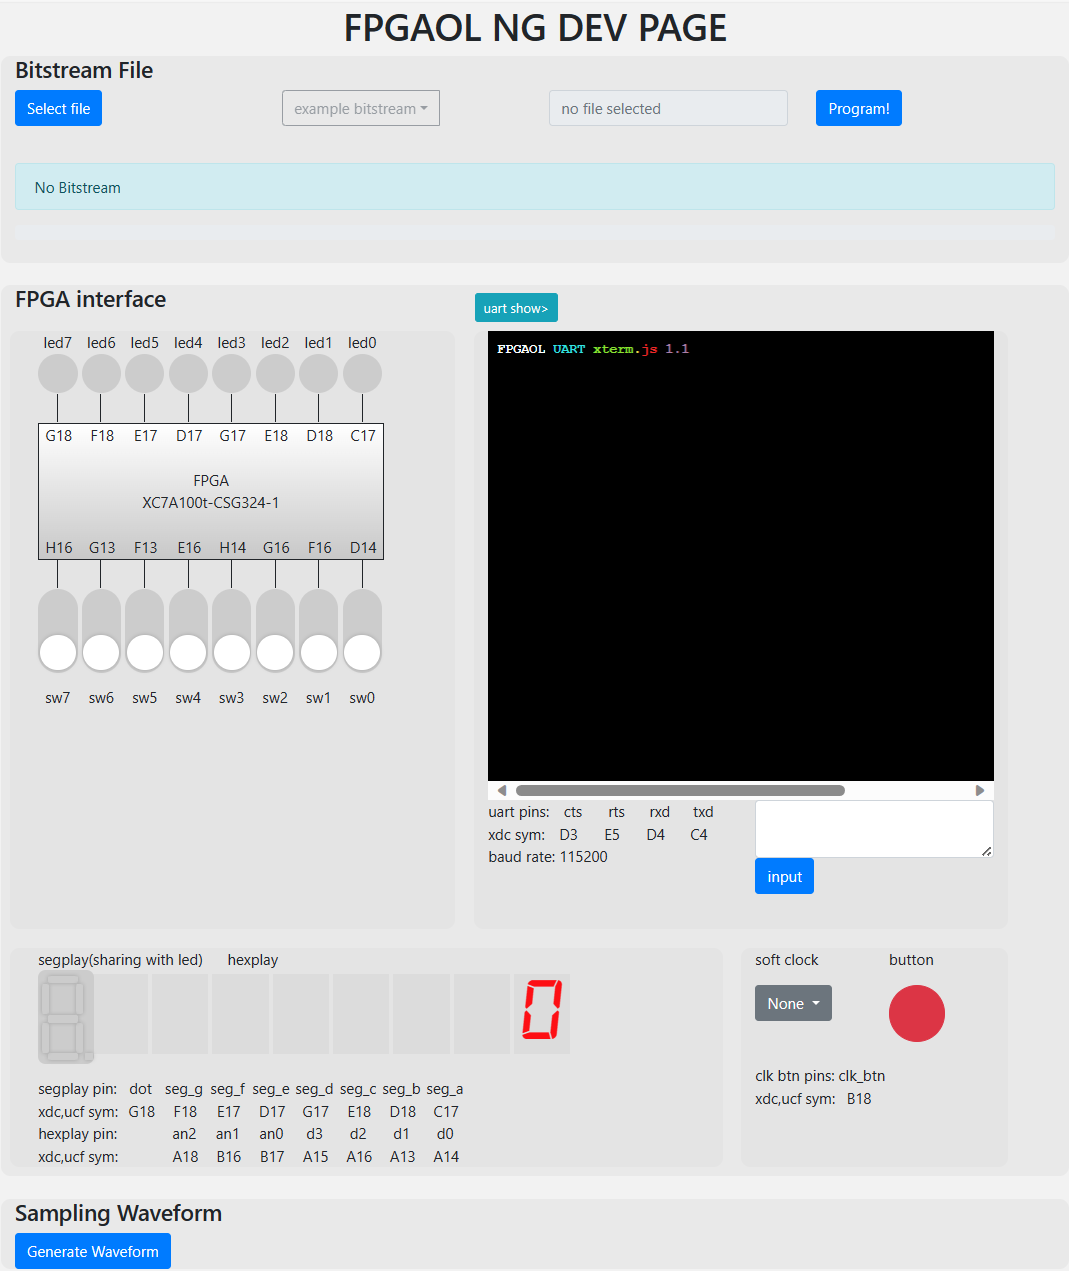
\includegraphics[width=0.8\textwidth]{lab0/35.png}
    \label{fig:35}
\end{figure}

在顶部点击"Select file"选择我们准备好的比特流文件进行上传,点击“Program”进行烧写。在提示“Program success!”之后,就可以通过网页上的外设接口与云端FPGA板卡进行交互。

\begin{figure}[H]
    \centering
    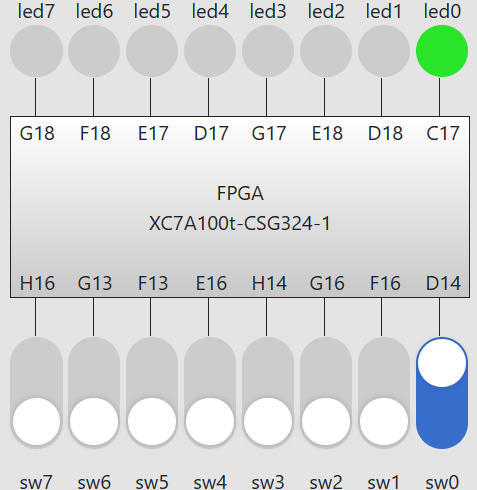
\includegraphics[width=0.35\textwidth]{lab0/36.png}
    \label{fig:36}
\end{figure}

\end{document}
